%%%%%%%%%%%%%%%%%%%%%%%%%%%%%%%%%%%%%%%%%%%%%%%%%%%%%%%%%%%%%%%%%%%%%%%%%%%%%%%
% Encoding: utf8
% Project: AIS - Exhibition ground - IS analysis and design
% Authors:
%     Libor Polčák, xpolca03@stud.fit.vutbr.cz
%     Boris Procházka, xproch63@stud.fit.vutbr.cz
%     Petr Zemek, xzemek02@stud.fit.vutbr.cz
% Description: Text of the third part of the project
%%%%%%%%%%%%%%%%%%%%%%%%%%%%%%%%%%%%%%%%%%%%%%%%%%%%%%%%%%%%%%%%%%%%%%%%%%%%%%%

\section*{Diagram případů použití}

\begin{figure}[H]
	\begin{center}
		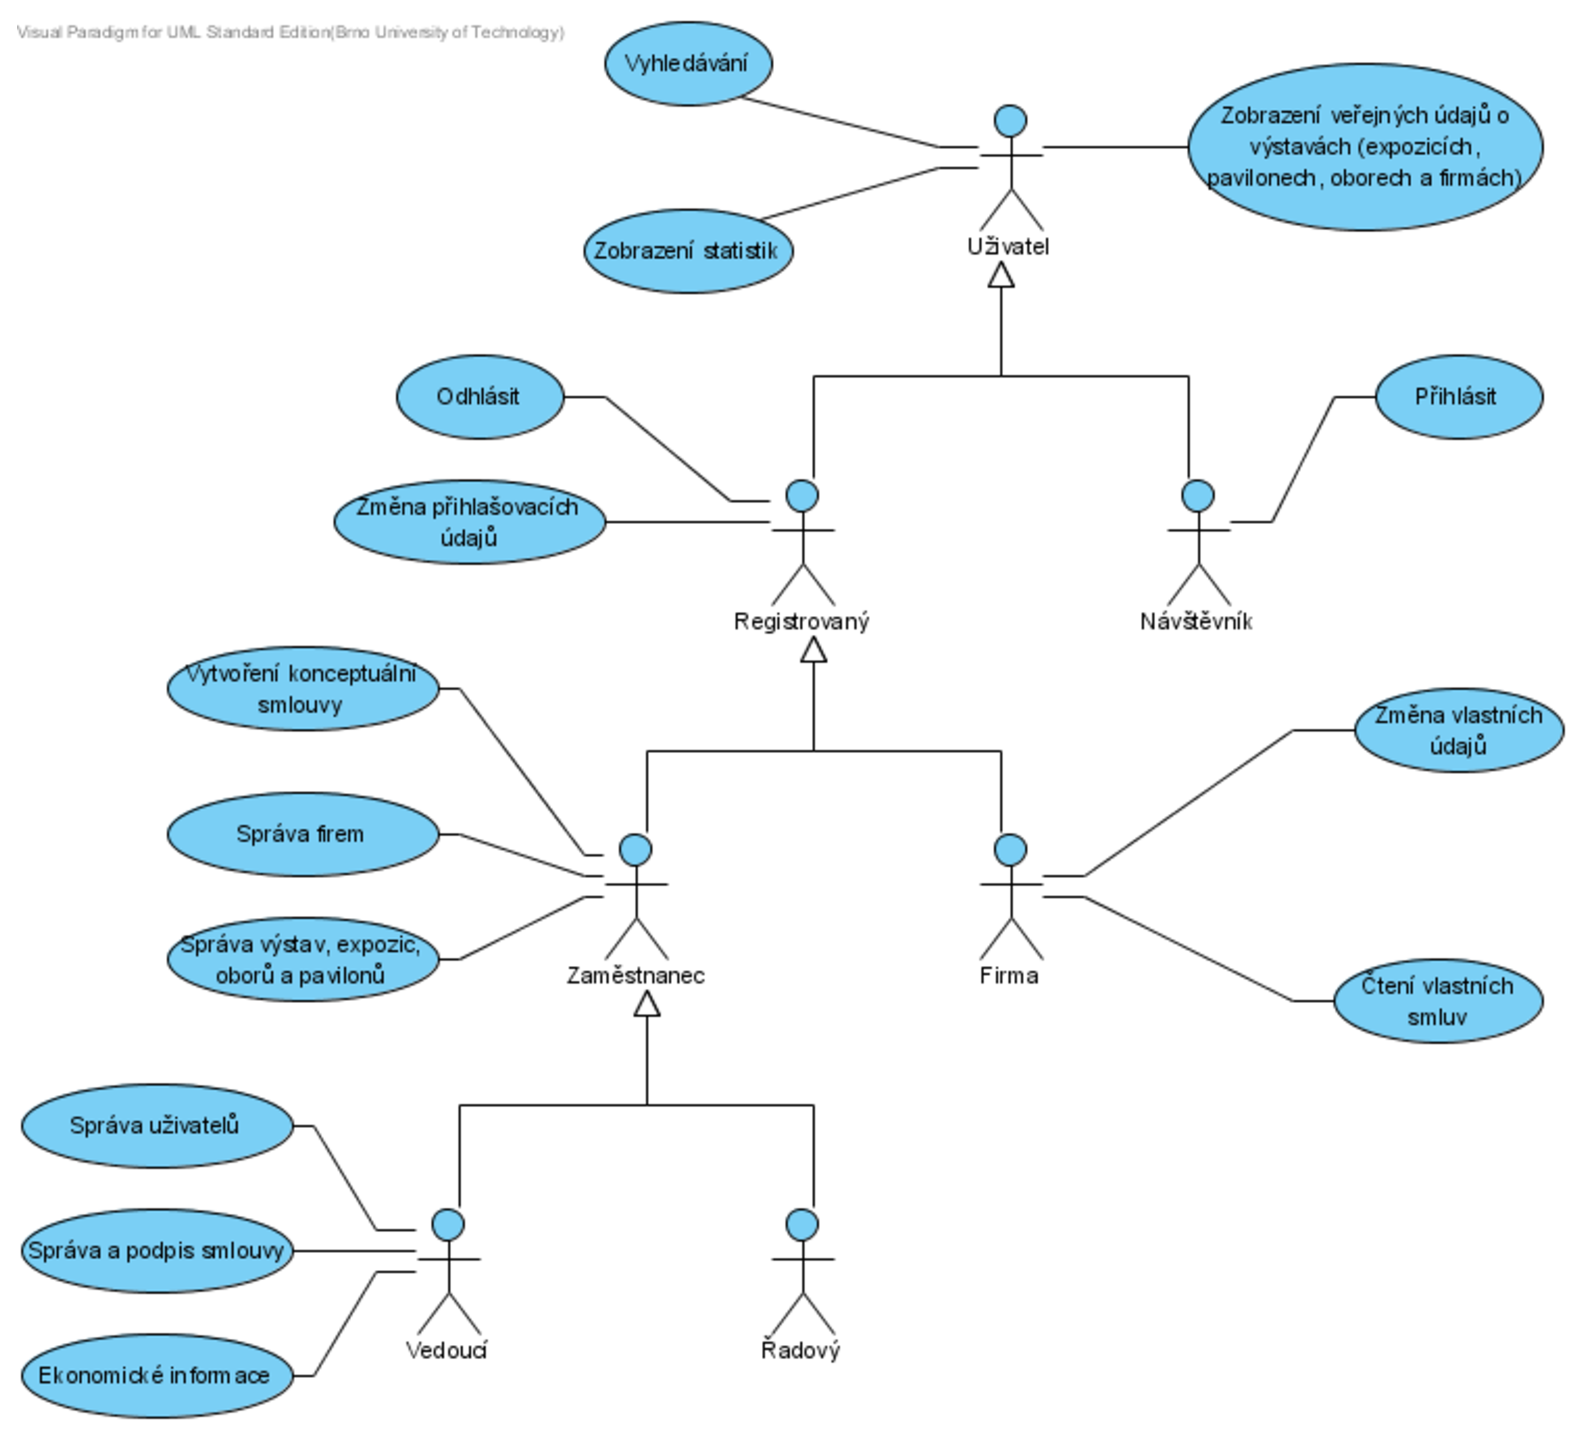
\includegraphics[width=12.5cm,keepaspectratio]{include/use_case_stage3}
	\end{center}
	\caption{Diagram případů použití}
\end{figure}

\section*{Specifikace případů použití}

\subsection*{Případ použití \uv{Vyhledávání}}

\begin{ais_table}
	\hline
	Název: & Vyhledávání \\

	\hline
	ID: & 4 \\

	\hline
	Stručný popis: & Uživatel vyhledává v~systému \\

	\hline
	Primární aktéři: & Uživatel \\

	\hline
	Sekundární aktéři: & \\

	\hline
	Předpoklady: &
		\begin{ais_table_first_enum}
			\item Žádné
		\end{ais_table_first_enum} \\

	\hline
	Akce pro spuštění: & Uživatel zvolí volbu \uv{Vyhledávání} \\

	\hline
	Hlavní tok: &
		\begin{ais_table_first_enum}
			\item Systém nabídne uživateli volbu následujících
			vyhledávacích kritérií:
				\begin{itemize}
					\item[--] vyhledávání výstav (dle názvu či intervalu, ve
					kterém se výstava má konat)
					\item[--] vyhledávání firem (dle názvu firmy či její adresy)
					\item[--] vyhledávání expozic (dle názvu expozice, jejího
					popisu, oboru či pavilonu, ve kterém se expozice nachází)
				\end{itemize}
			\item Uživatel vyplní vyhledávací kritéria
			\item Uživatel potvrdí zadaná kritéria
			\item Systém uživateli zobrazí výsledky vyhledávání dle zvolených
			kritérií
		\end{ais_table_first_enum} \\

	\hline
	Následné podmínky: &
		\begin{ais_table_first_enum}
			\item Jsou zobrazeny výsledky vyhledávání
		\end{ais_table_first_enum} \\

	\hline
	Alternativní toky: & Žádné \\

	\hline
	Výjimky: & Storno \\
	         & Selhání operace \\
	         & Selhání systému \\

	\hline
	Speciální požadavky: &
		\begin{ais_table_first_enum}
			\item Zobrazené výsledky vyhledávání budou umožňovat zobrazení
			detailů o~vyhledaných objektech (např. v~seznamu výstav, která
			vyhovovala zadaným kritériím, budou zobrazeny odkazy na detaily
			těchto výstav)
			\item U~zadávání oboru expozice při vyhledávání expozic systém
			nabídne uživateli výběr existujících oborů
		\end{ais_table_first_enum} \\

	\hline
\end{ais_table}

\subsubsection*{Výjimky případu použití \uv{Vyhledávání}}

Výjimky případu použití \uv{Vyhledávání} odpovídají (po úpravách) výjimkám
případu použití 1.

\subsection*{Případ použití \uv{Vytvoření konceptuální smlouvy}}

\begin{ais_table}
	\hline
	Název: & Vytvoření konceptuální smlouvy \\

	\hline
	ID: & 5 \\

	\hline
	Stručný popis: & Zaměstnanec výstaviště vytvoří nepodepsanou smlouvu \\

	\hline
	Primární aktéři: & Zaměstnanec \\

	\hline
	Sekundární aktéři: & \\

	\hline
	Předpoklady: &
		\begin{ais_table_first_enum}
			\item Uživatel je přihlášený do systému jako zaměstnanec
		\end{ais_table_first_enum} \\

	\hline
	Akce pro spuštění: & Uživatel zvolí \uv{Vytvořit novou konceptuální smlouvu} \\

	\hline
	Hlavní tok: &
		\begin{ais_table_first_enum}
			\item Spustí se okno vytváření konceptuální smlouvy
				\begin{enumerate*}
					\item[1.1.] Uživatel vybere firmu, se kterou se bude uzavírat smlouva
					\item[1.2.] Uživatel nastaví datum splatnosti (má k~dispozici
						přehledný kalendář)
					\item[1.3.] Systém vloží do databáze konceptuální smlouvu
					\item[1.4.] Uživatel má možnost přidat ke smlouvě expozici (viz případ užití 6)
					\item[1.5.] Uživatel potvrdí zadané údaje
				\end{enumerate*}
			\item Systém spočítá průběžnou cenu pro smlouvu
		\end{ais_table_first_enum} \\

	\hline
	Následné podmínky: &
		\begin{ais_table_first_enum}
			\item Smlouva uložená v~databází se všemi náležitostmi
		\end{ais_table_first_enum} \\

	\hline
	Alternativní toky: & \\

	\hline
	Výjimky: & Storno \\
	         & Selhání operace \\
	         & Selhání systému \\

	\hline
\end{ais_table}

\subsubsection*{Výjimky případu použití \uv{Vytvoření konceptuální smlouvy}}

Výjimky případu použití \uv{Vytvoření konceptuální smlouvy} odpovídají (po
úpravách) výjimkám případu použití 1.

\subsection*{Případ použití \uv{Vytvoření nové expozice}}

\begin{ais_table}
	\hline
	Název: & Vytvoření nové expozice \\

	\hline
	ID: & 6 \\

	\hline
	Stručný popis: & Zaměstnanec výstaviště vytvoří novou expozici \\

	\hline
	Primární aktéři: & Zaměstnanec \\

	\hline
	Sekundární aktéři: & \\

	\hline
	Předpoklady: &
		\begin{ais_table_first_enum}
			\item Uživatel je přihlášený do systému jako zaměstnanec
			\item Je zobrazena nepodepsaná smlouva
			\item Je vybrána výstava, do které se expozice bude přidávat
		\end{ais_table_first_enum} \\

	\hline
	Akce pro spuštění: & Uživatel zvolí \uv{Přidat další (expozici)}  \\

	\hline
	Hlavní tok: &
		\begin{ais_table_first_enum}
			\item Spustí se okno přidání expozice
				\begin{enumerate*}
					\item[1.2.] Uživatel vybere pavilón, ve kterém bude expozice
					\item[1.3.] Uživatel vybere obor, ke kterému se bude expozice vztahovat
					\item[1.4.] Uživatel zadá plochu, kterou bude expozice zabírat.
						Volitelně může zadat název a popis expozice
					\item[1.5.] Uživatel potvrdí zadané údaje
				\end{enumerate*}
			\item Systém spočítá cenu expozice
			\item Systém navýší cenu u~smlouvy
			\item Systém vloží do databáze expozici
		\end{ais_table_first_enum} \\

	\hline
	Následné podmínky: &
		\begin{ais_table_first_enum}
			\item Expozice je uložená v~databázi
			\item Cena smlouvy je navýšena o~cenu expozice
		\end{ais_table_first_enum} \\

	\hline
	Alternativní toky: & V~pavilónu není dostatek místa pro expozici \\

	\hline
	Výjimky: & Storno \\
	         & Selhání operace \\
	         & Selhání systému \\

	\hline
\end{ais_table}

\subsubsection*{Alternativní toky případu použití \uv{Vytvoření nové expozice}}

\begin{ais_table}
	\hline
	Název: & Vytvoření nové expozice: V~pavilónu není dostatek místa pro expozici \\

	\hline
	ID: & 6.1 \\

	\hline
	Stručný popis: & Systém informuje uživatele, že v~pavilónu není dostatek místa
	pro vložení expozice\\

	\hline
	Primární aktéři: & Zaměstnanec \\

	\hline
	Sekundární aktéři: & \\

	\hline
	Předpoklady: &
		\begin{ais_table_first_enum}
			\item Součet plochy již rezervovaných expozic (pro danou výstavu a
				pavilón) je s~nově přidávanou expozicí větší, než je rozloha pavilónu
		\end{ais_table_first_enum} \\

	\hline
	Akce pro spuštění: & Uživatel v~kroku 1.4 hlavního toku případu užití 6
	zadá příliš velkou plochu expozice \\

	\hline
	Alternativní tok: &
		\begin{ais_table_first_enum}
			\item Systém uživatele upozorní, že expozici nelze do pavilónu umístit
			\item Návrat k~bodu 1.4 hlavního toku
		\end{ais_table_first_enum} \\

	\hline
\end{ais_table}

\subsubsection*{Výjimky případu použití \uv{Vytvoření nové expozice}}

Výjimky případu použití \uv{Vytvoření nové expozice} odpovídají (po úpravách)
výjimkám případu použití 1.

\subsection*{Případ použití \uv{Čtení vlastních smluv}}

\begin{ais_table}
	\hline
	Název: & Čtení vlastních smluv \\

	\hline
	ID: & 7\\

	\hline
	Stručný popis: & Firma může číst obsah vlastních smluv\\

	\hline
	Primární aktéři: & Firma\\

	\hline
	Sekundární aktéři: & \\

	\hline
	Předpoklady: &
		\begin{ais_table_first_enum}
			\item Uživatel je do systému přihlášen jako firma
			\item Firma uzavřela s~výstavištěm alespoň jednu smlouvu
		\end{ais_table_first_enum} \\

	\hline
	Akce pro spuštění: & Uživatel zvolí \uv{čtení smlouvy ČÍSLO\_SMLOUVY}\\

	\hline
	Hlavní tok: &
		\begin{ais_table_first_enum}
			\item Smluvní informace jsou načteny ze systému
			\item Smluvní informace jsou zobrazeny
			\item Systém zobrazí aktuální stav kontraktu
		\end{ais_table_first_enum} \\

	\hline
	Následné podmínky: &
		\begin{ais_table_first_enum}
			\item Žádné
		\end{ais_table_first_enum} \\

	\hline
	Alternativní toky: & Žádné\\

	\hline
	Výjimky: & Storno \\
	         & Selhání operace \\
	         & Selhání systému \\

	\hline
\end{ais_table}

\subsubsection*{Výjimky případu použití \uv{Čtení vlastních smluv}}

Výjimky případu použití \uv{Čtení vlastních smluv} odpovídají (po úpravách)
výjimkám případu použití 1.


\pagebreak

\section*{Konceptuální diagram tříd}

\begin{figure}[H]
	\begin{center}
		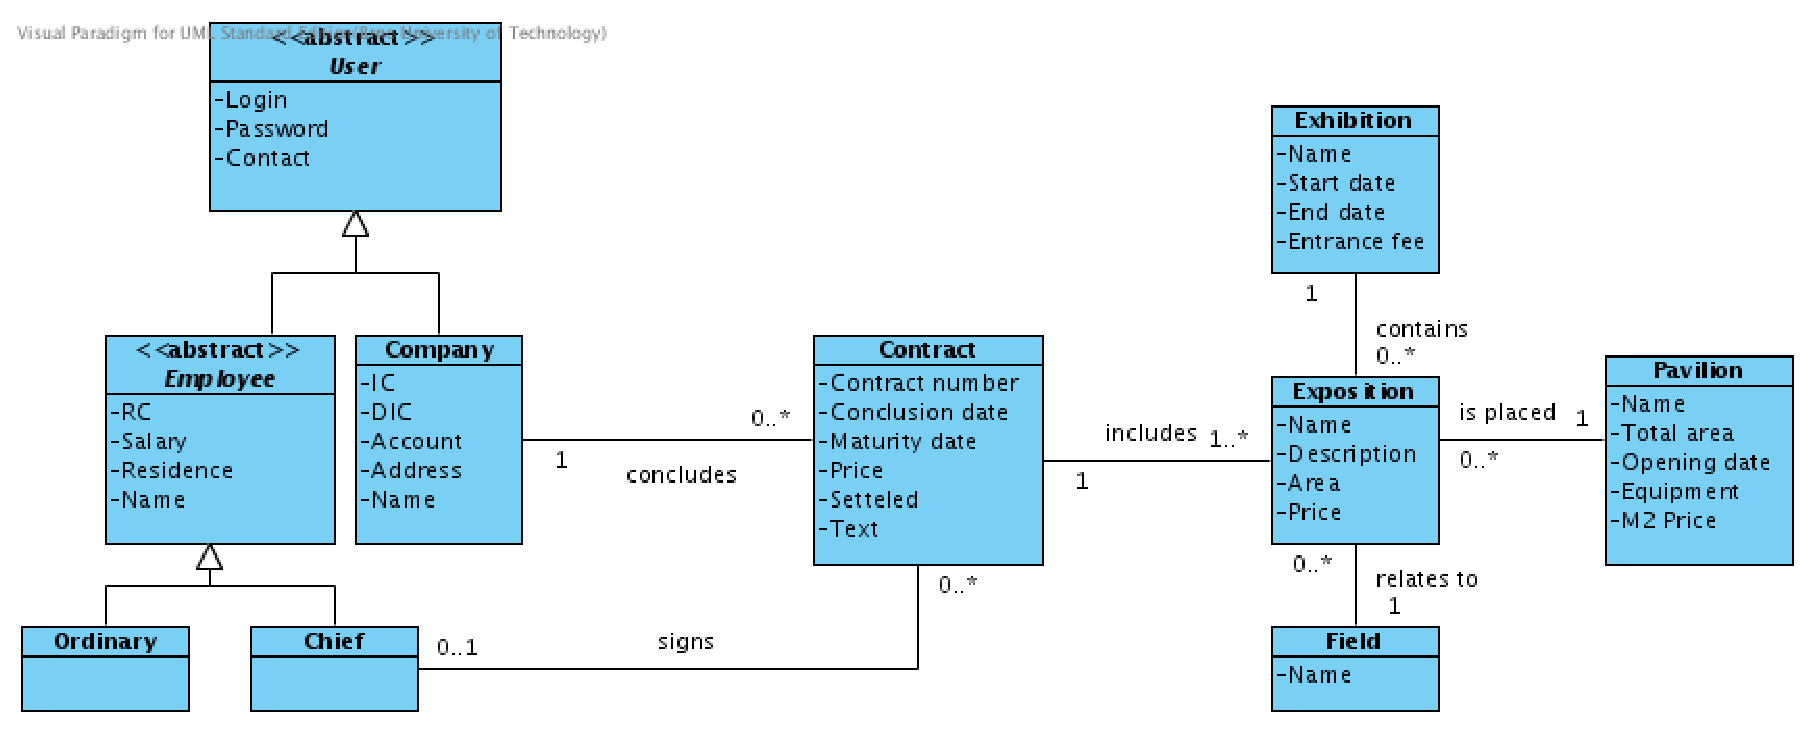
\includegraphics[width=16cm,keepaspectratio]{include/conceptual_final}
	\end{center}
	\caption{Konceptuální diagram tříd}
	\label{fig:ConceptualFinal}
\end{figure}

\pagebreak

\section*{Návrh schématu databáze}

\begin{figure}[H]
	\begin{center}
		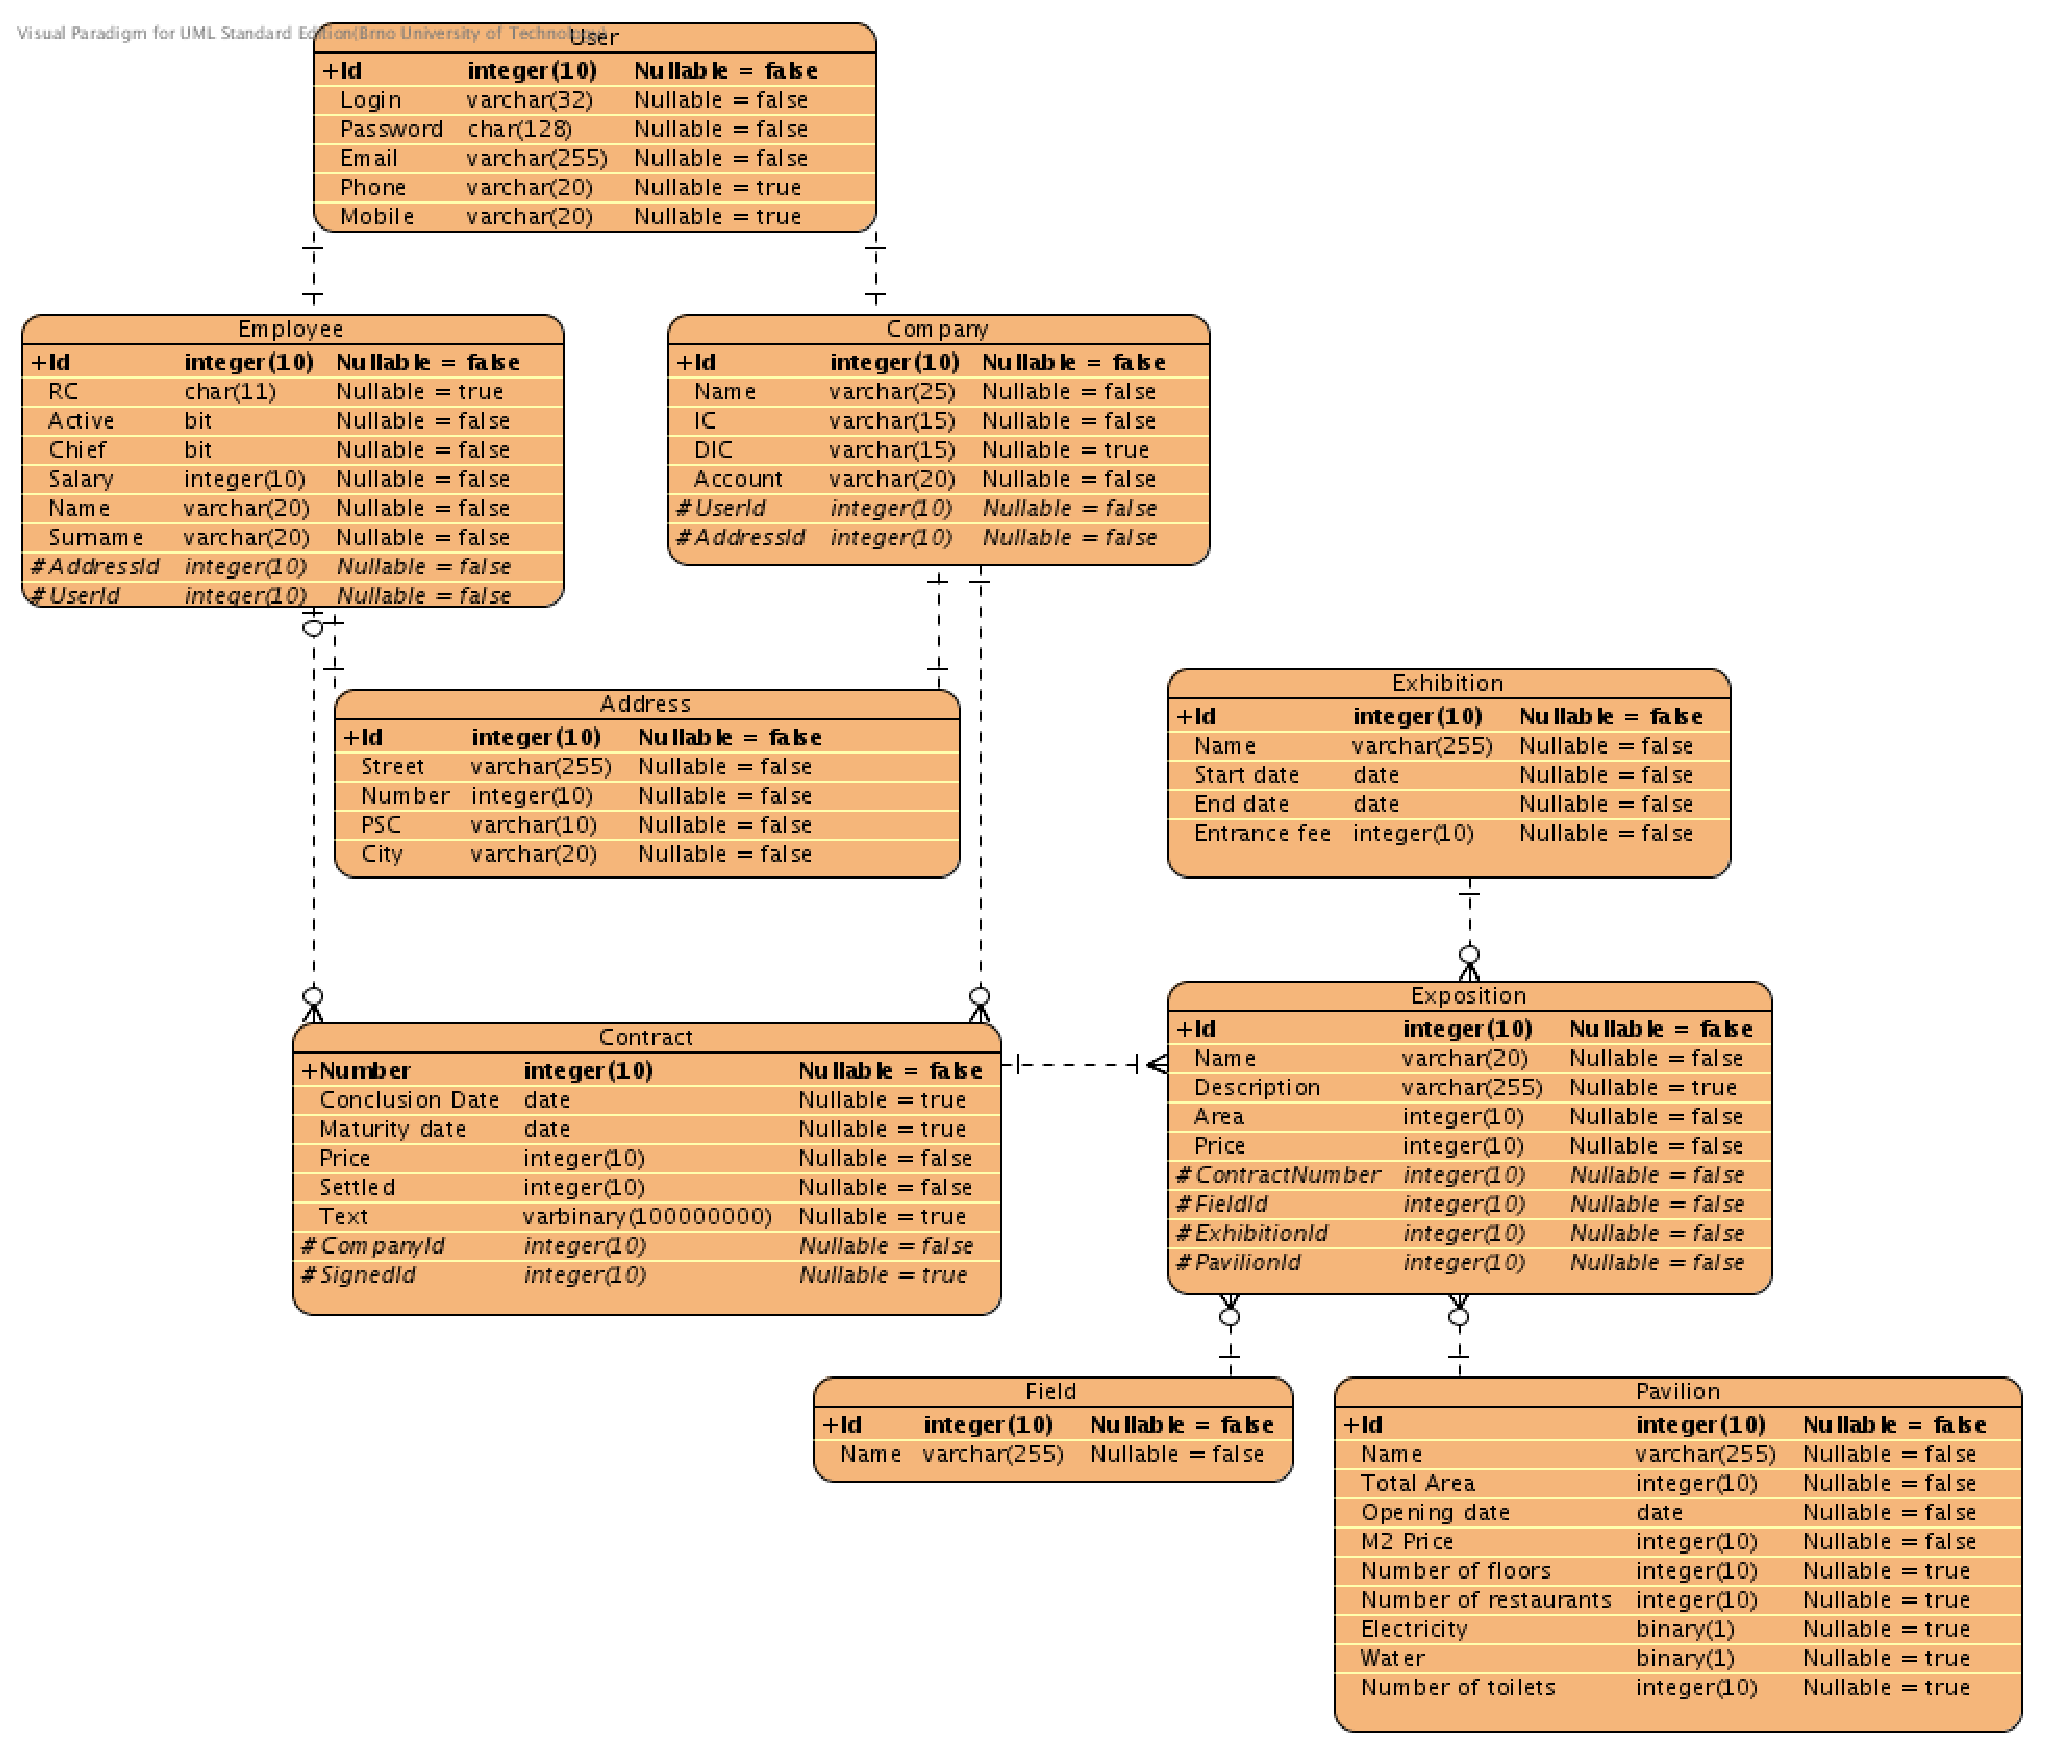
\includegraphics[width=16cm,keepaspectratio]{include/schema_final}
	\end{center}
	\caption{Návrh schématu databáze}
	\label{fig:SchemaFinal}
\end{figure}

\pagebreak

\section*{Diagram návrhových tříd}

\begin{figure}[H]
	\begin{adjustwidth}{-4cm}{-4cm}
		\begin{center}
			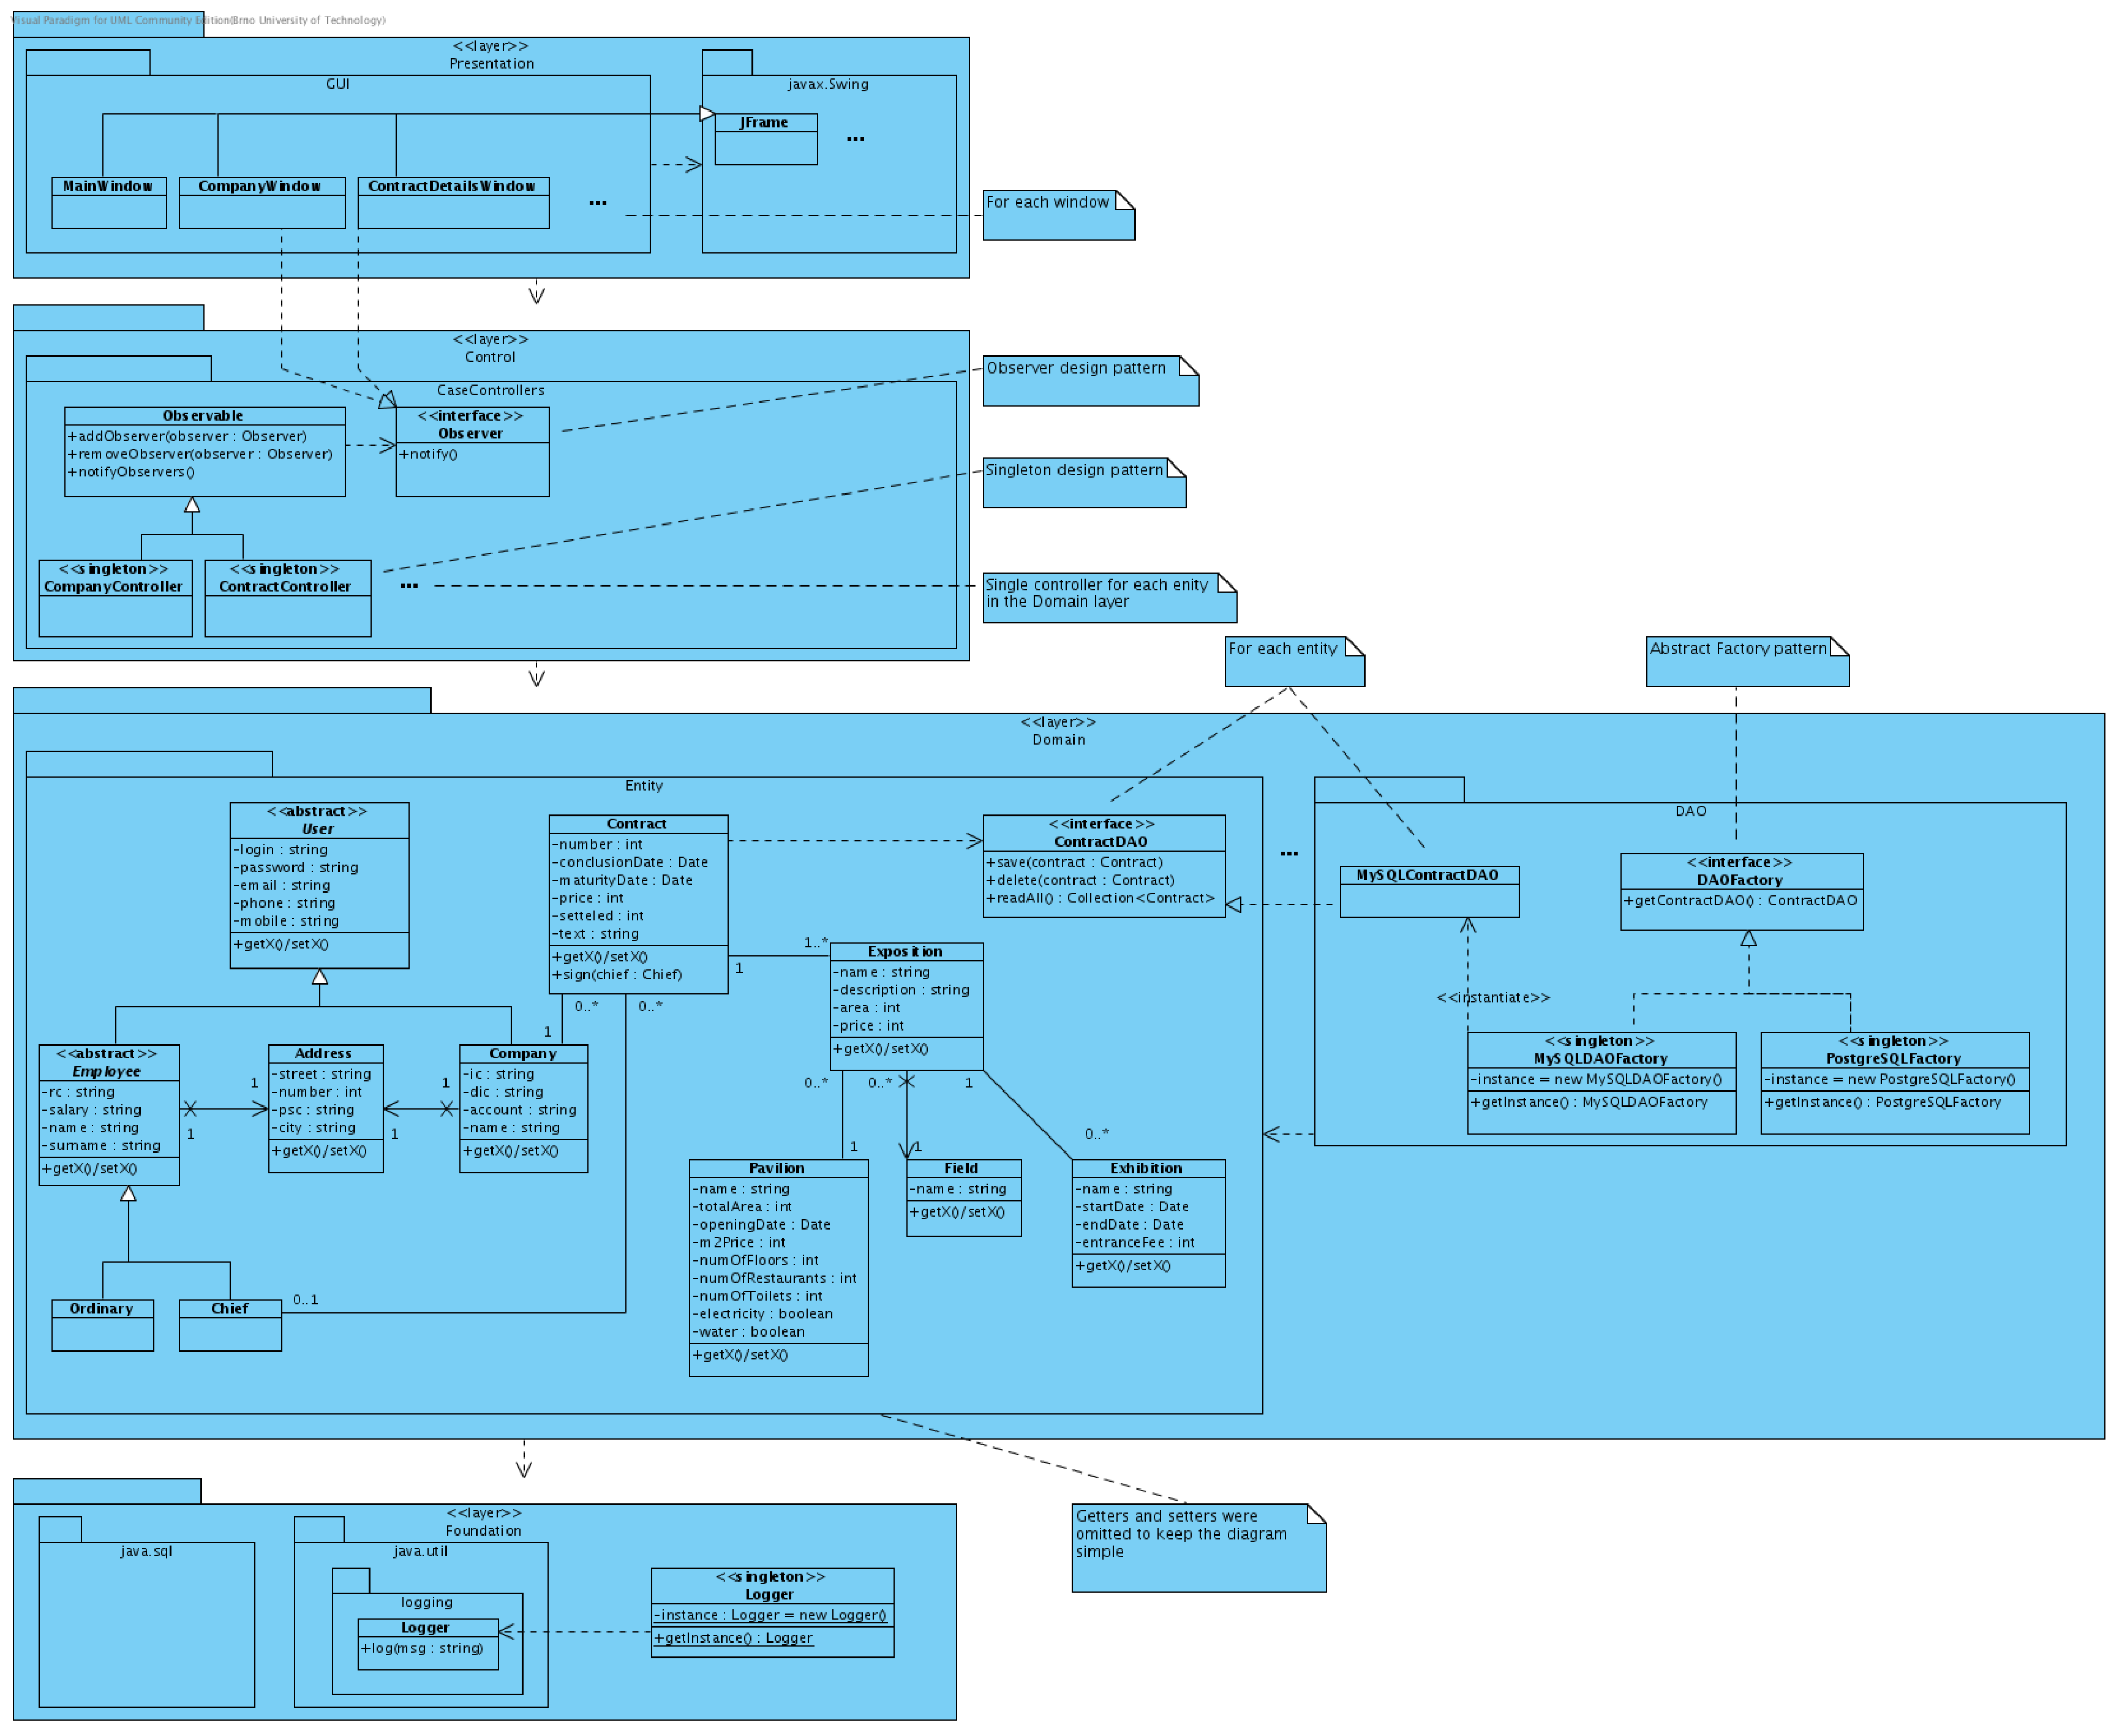
\includegraphics[width=20cm,keepaspectratio]{include/class_final}
		\end{center}
	\end{adjustwidth}
	\caption{Diagram návrhových tříd}
	\label{fig:ClassFinal}
\end{figure}

\pagebreak

\section*{Diagramy interakce}

\begin{figure}[H]
	\begin{center}
		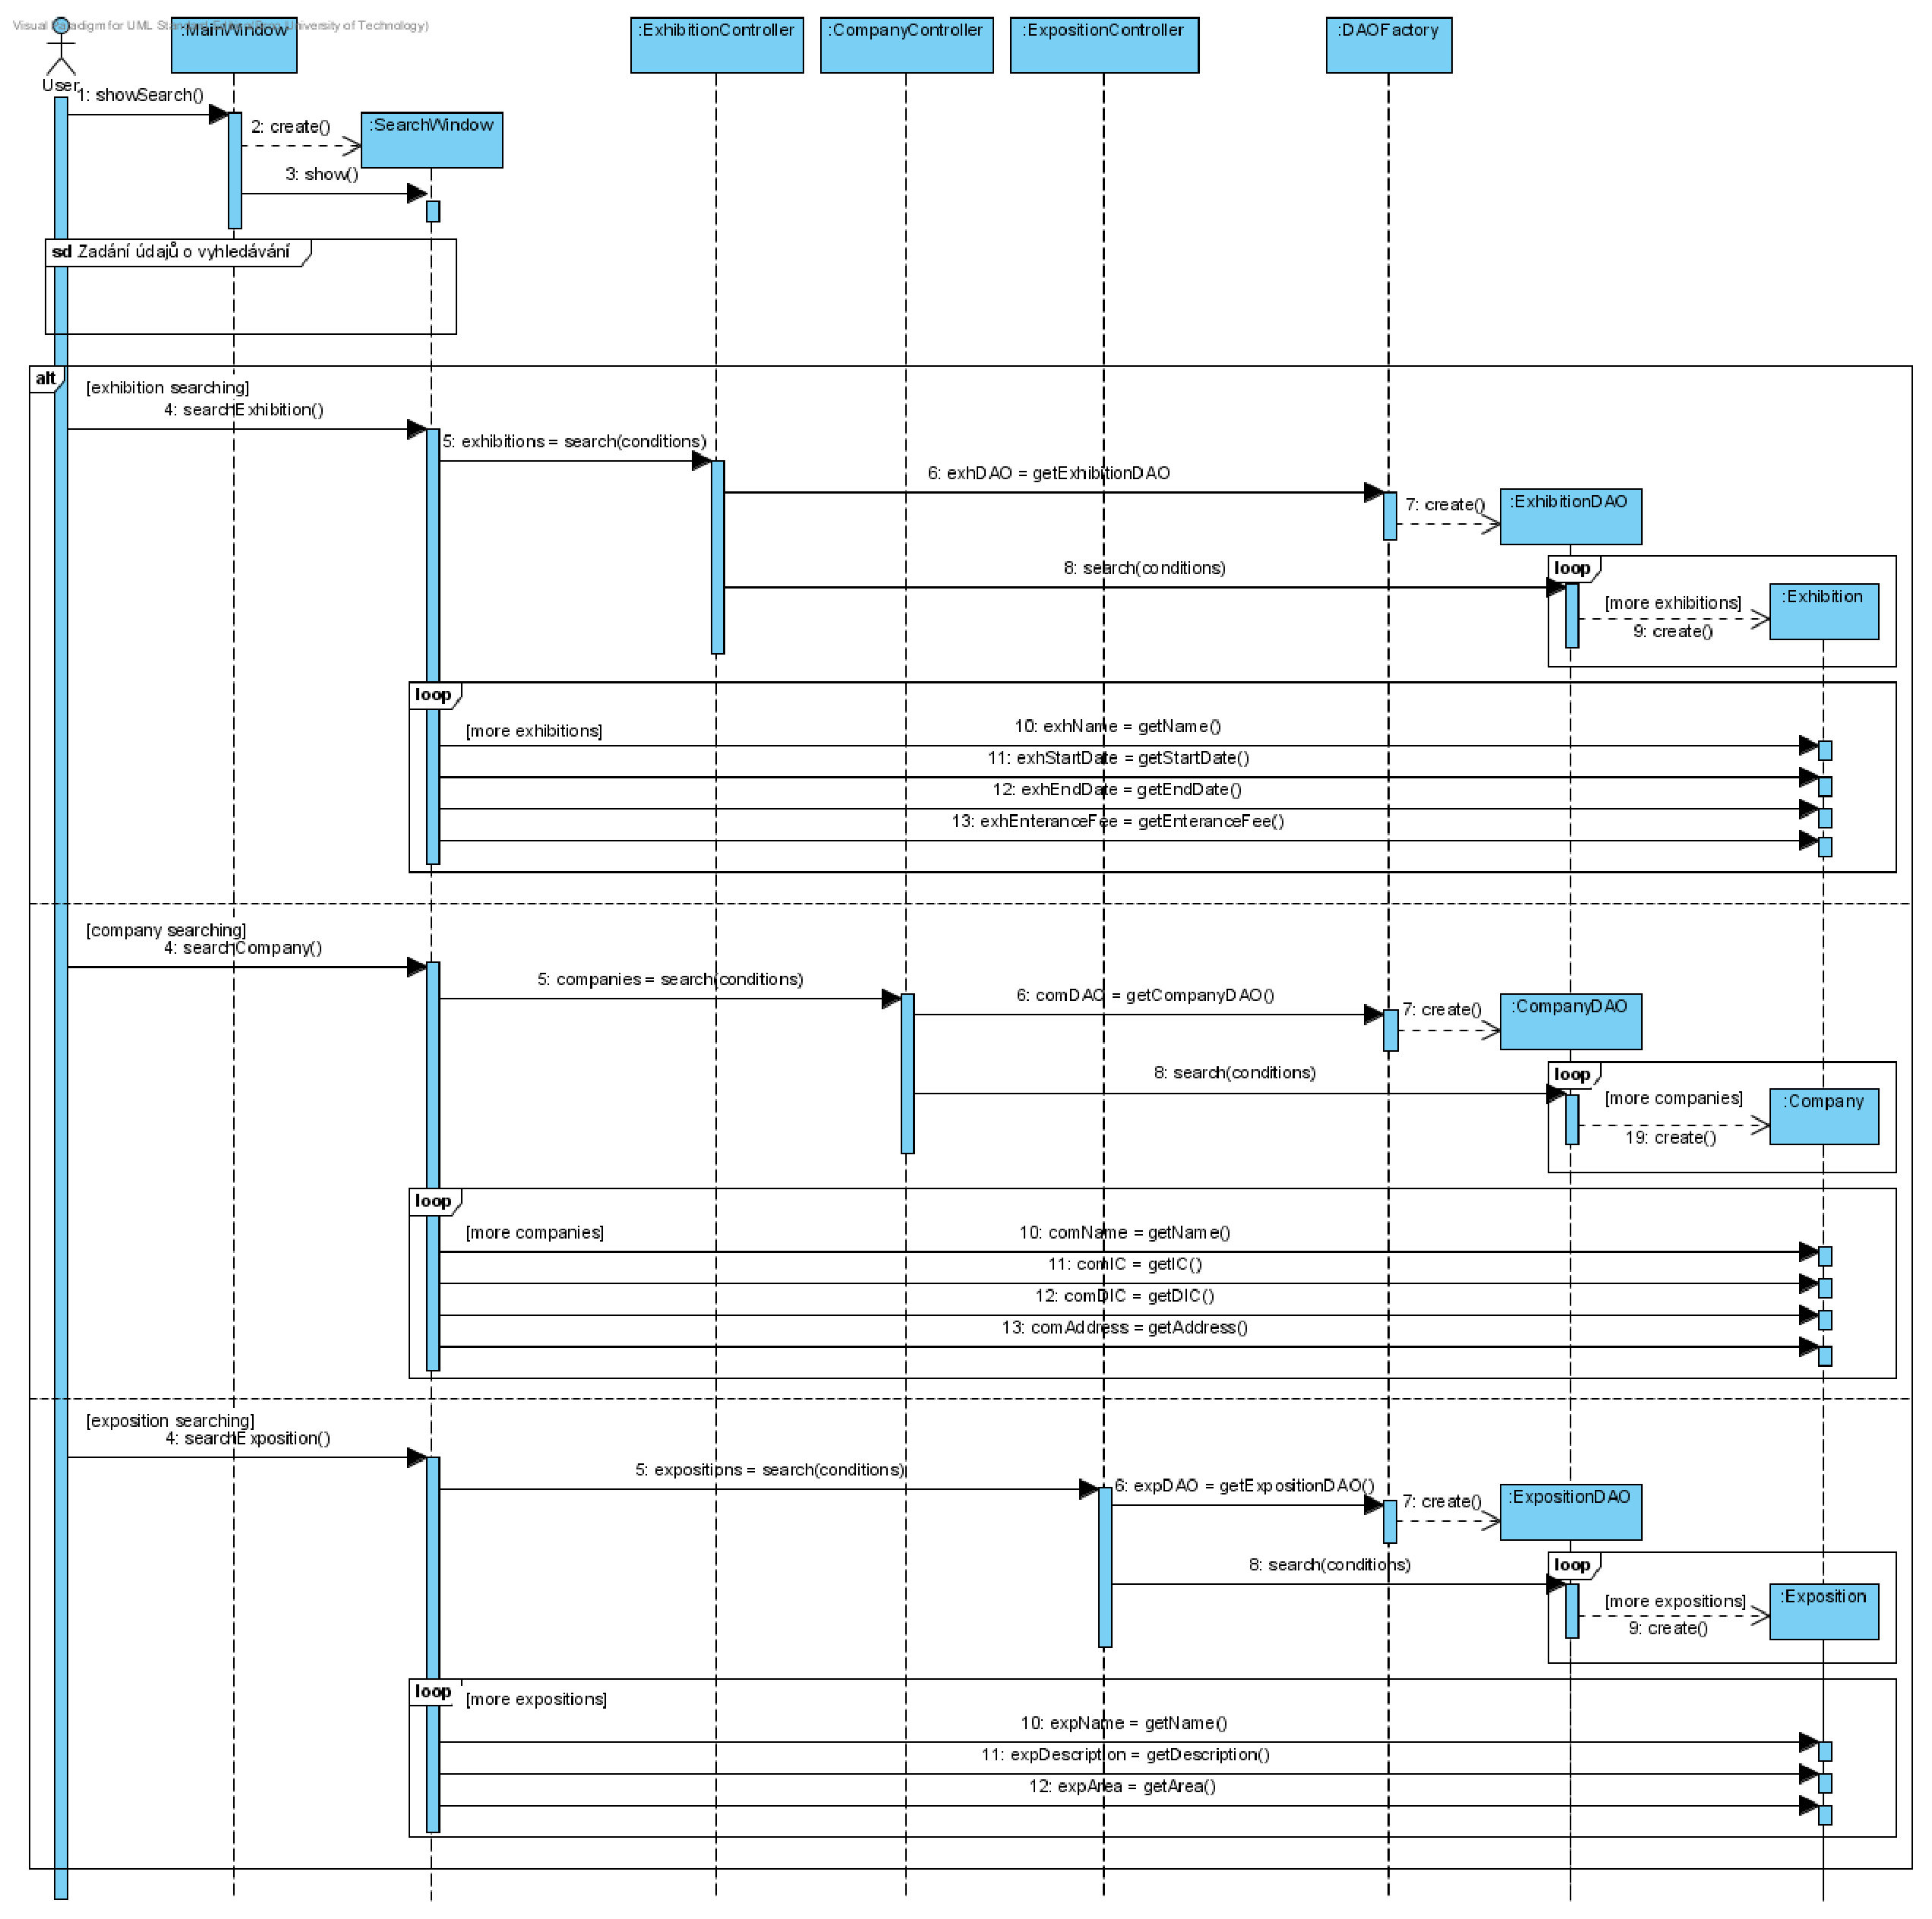
\includegraphics[width=16cm,keepaspectratio]{include/seq_search}
	\end{center}
	\caption{Diagram sekvence k~případu použití \uv{Vyhledávání}}
	\label{fig:SeqSearch}
\end{figure}

\pagebreak

\begin{landscape}
\begin{figure}[H]
	\begin{center}
		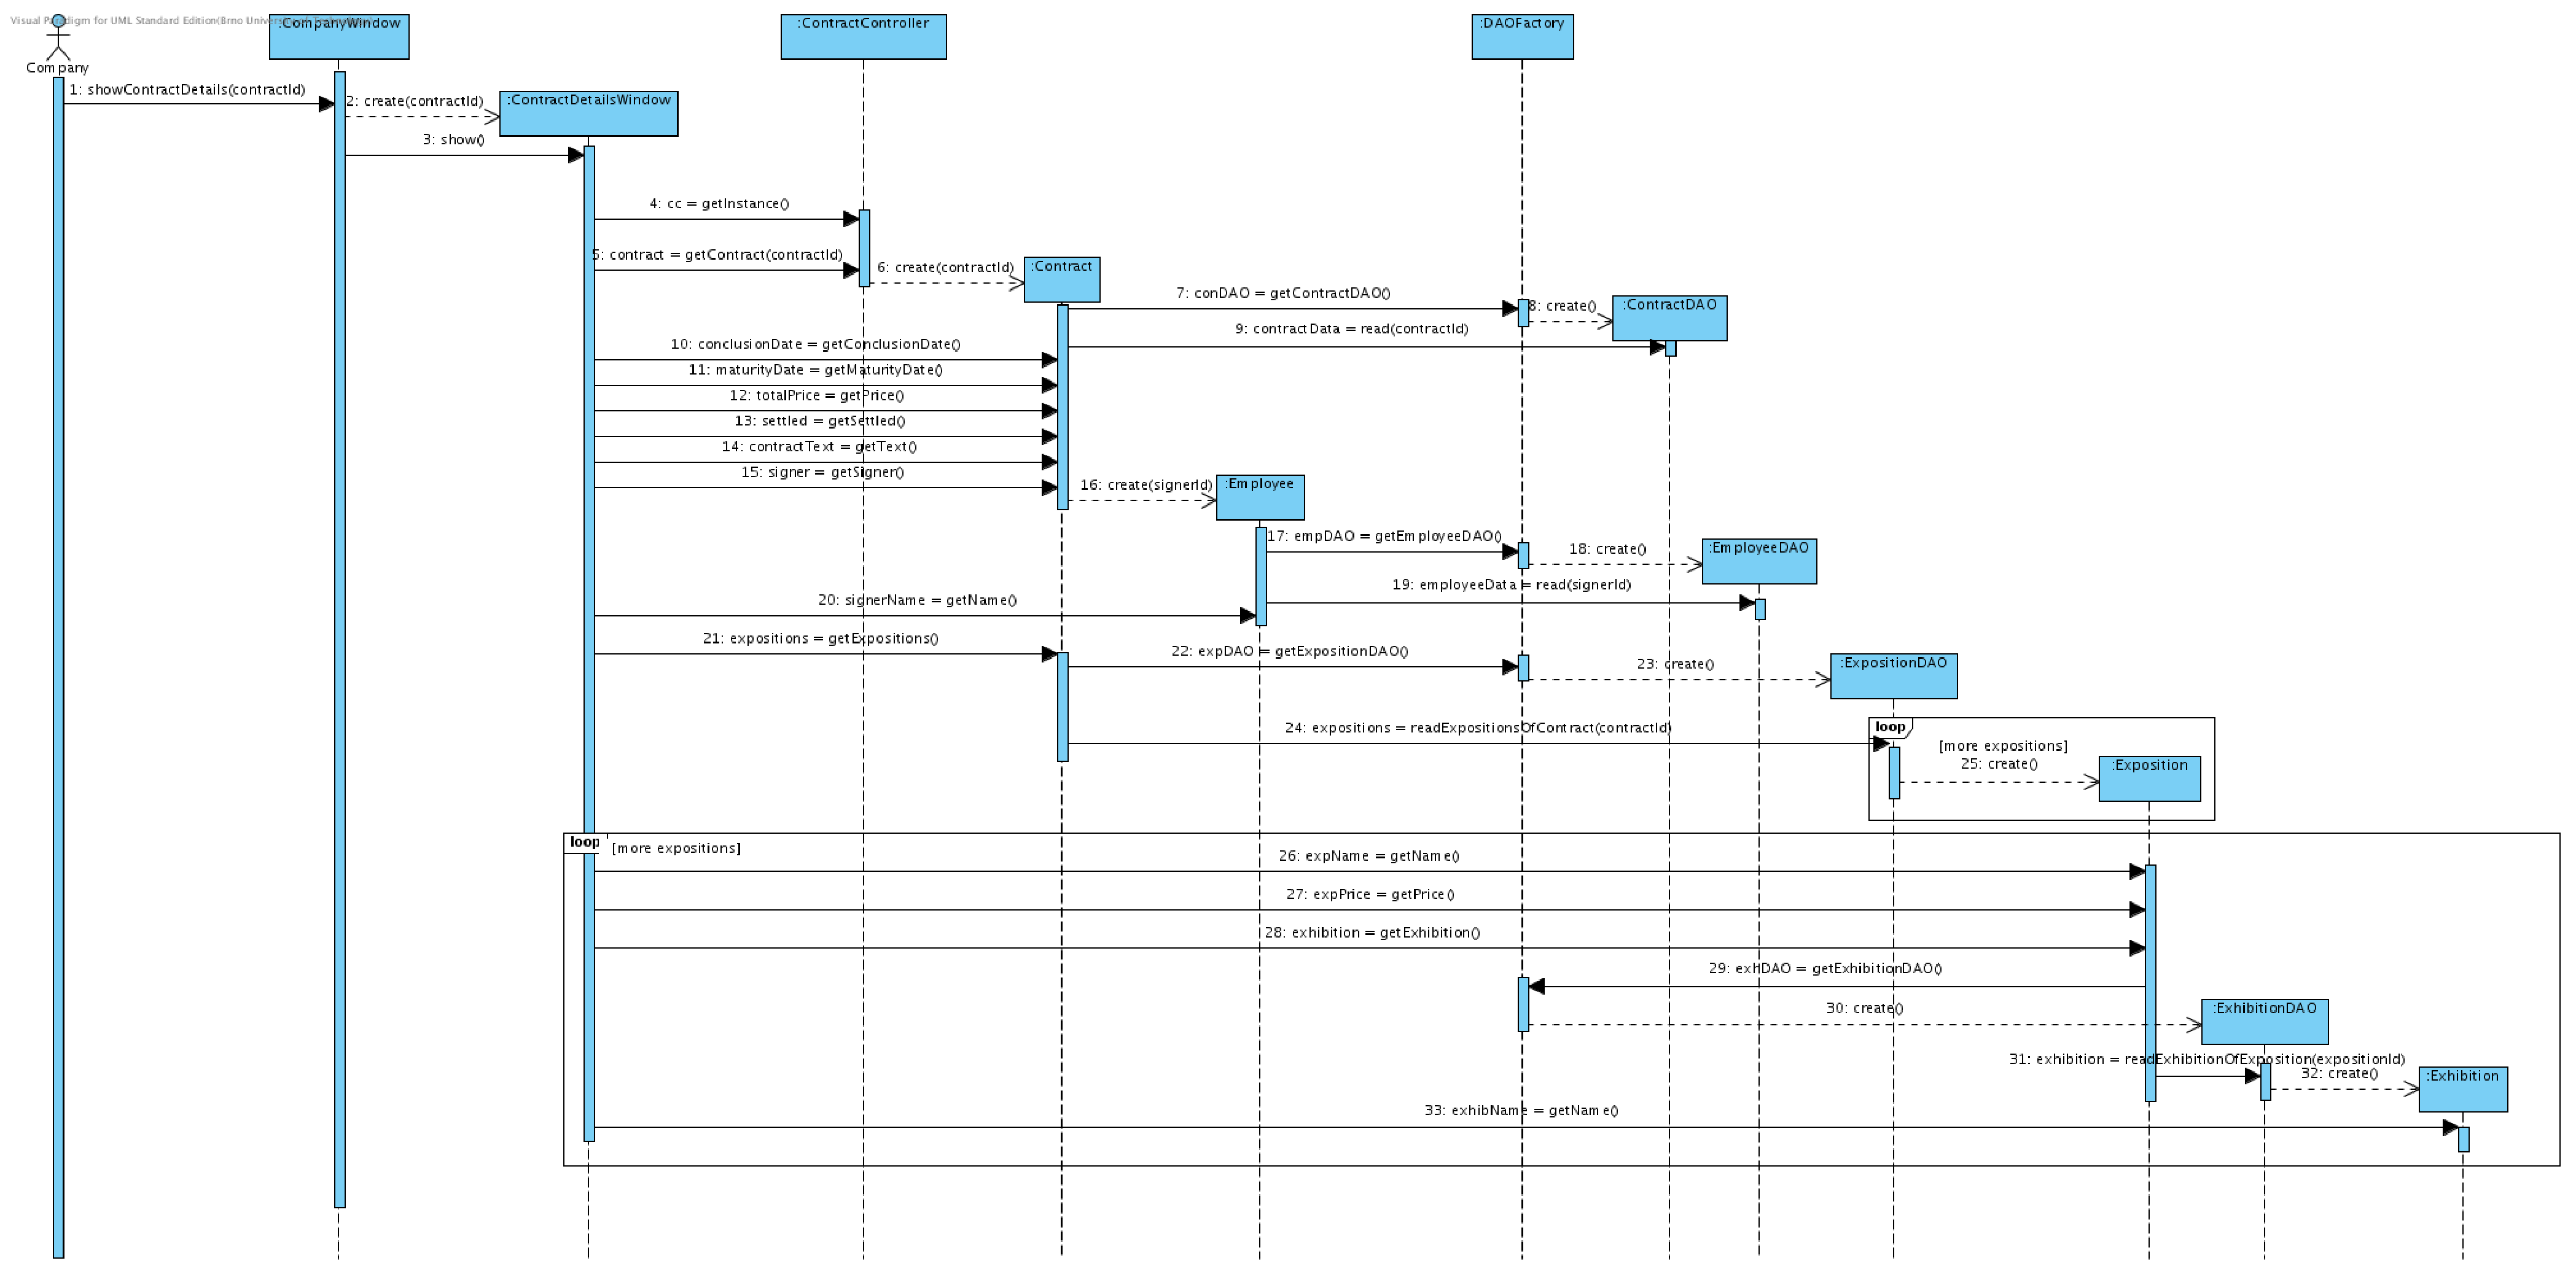
\includegraphics[width=25cm,keepaspectratio]{include/seq_read_own_contract}
	\end{center}
	\caption{Diagram sekvence k~případu použití \uv{Čtení vlastní smlouvy}}
	\label{fig:SeqReadOwnContract}
\end{figure}
\end{landscape}

\pagebreak

\section*{Diagramy návaznosti obrazovek}

Z~důvodu zvýšení přehlednosti diagramů neobsahují názvy obrázek příponu
\uv{Window}, která je u~všech názvů brána jako implicitní.

\begin{figure}[h]
	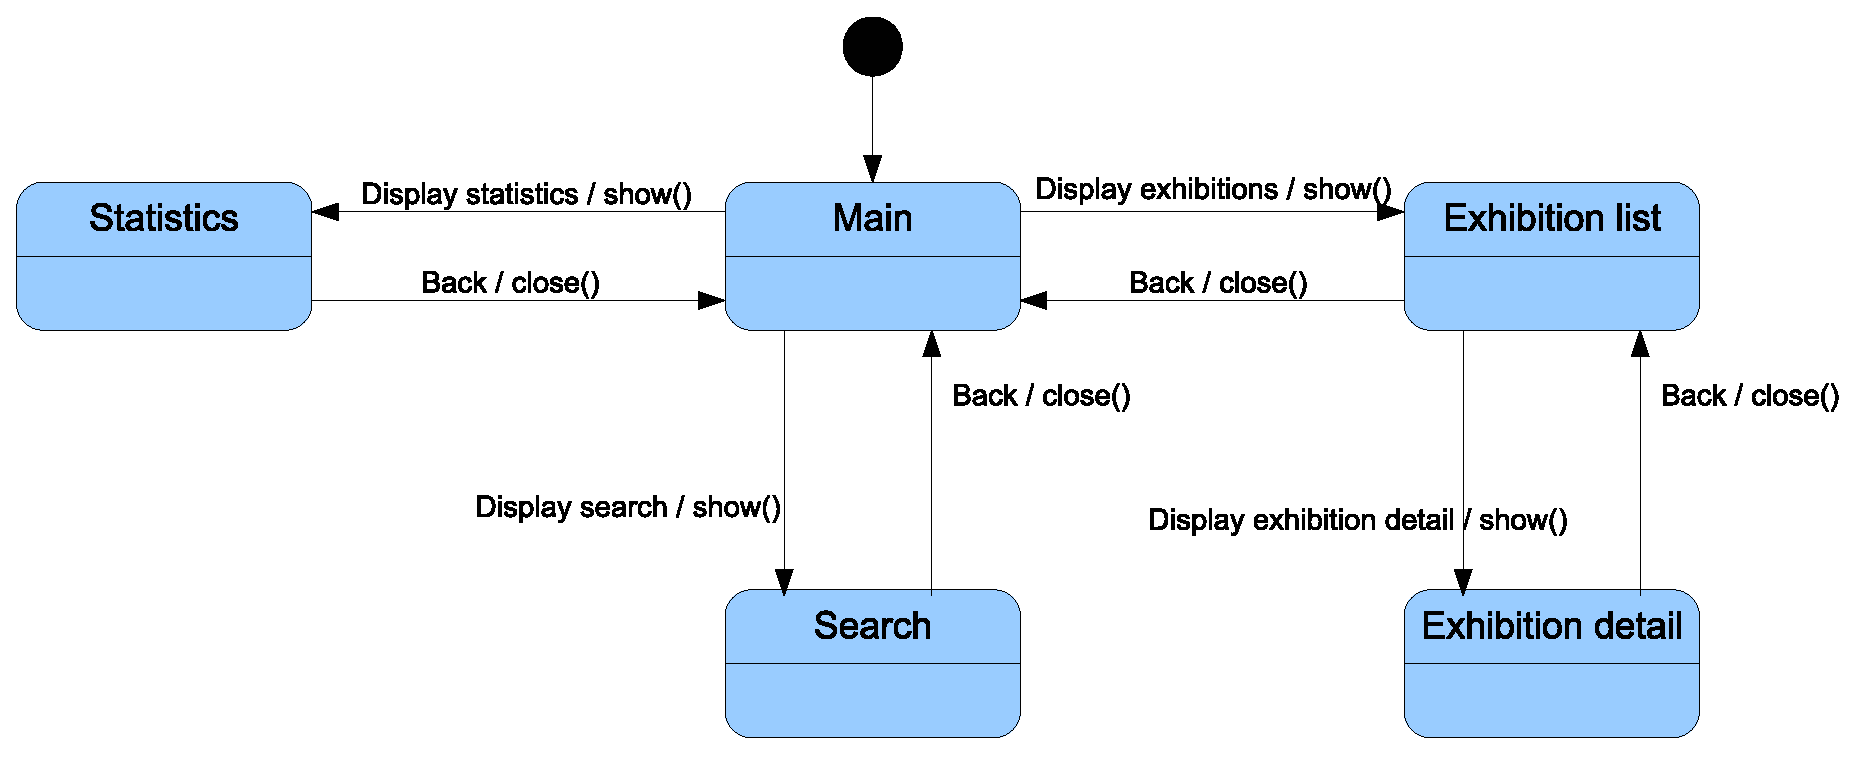
\includegraphics[width=13cm,keepaspectratio]{include/screens_role_user}
	\caption{Stavový diagram návaznosti obrazovek pro roli \uv{Uživatel}}
	\label{fig:ScreensRoleUser}
\end{figure}

\begin{figure}[h]
	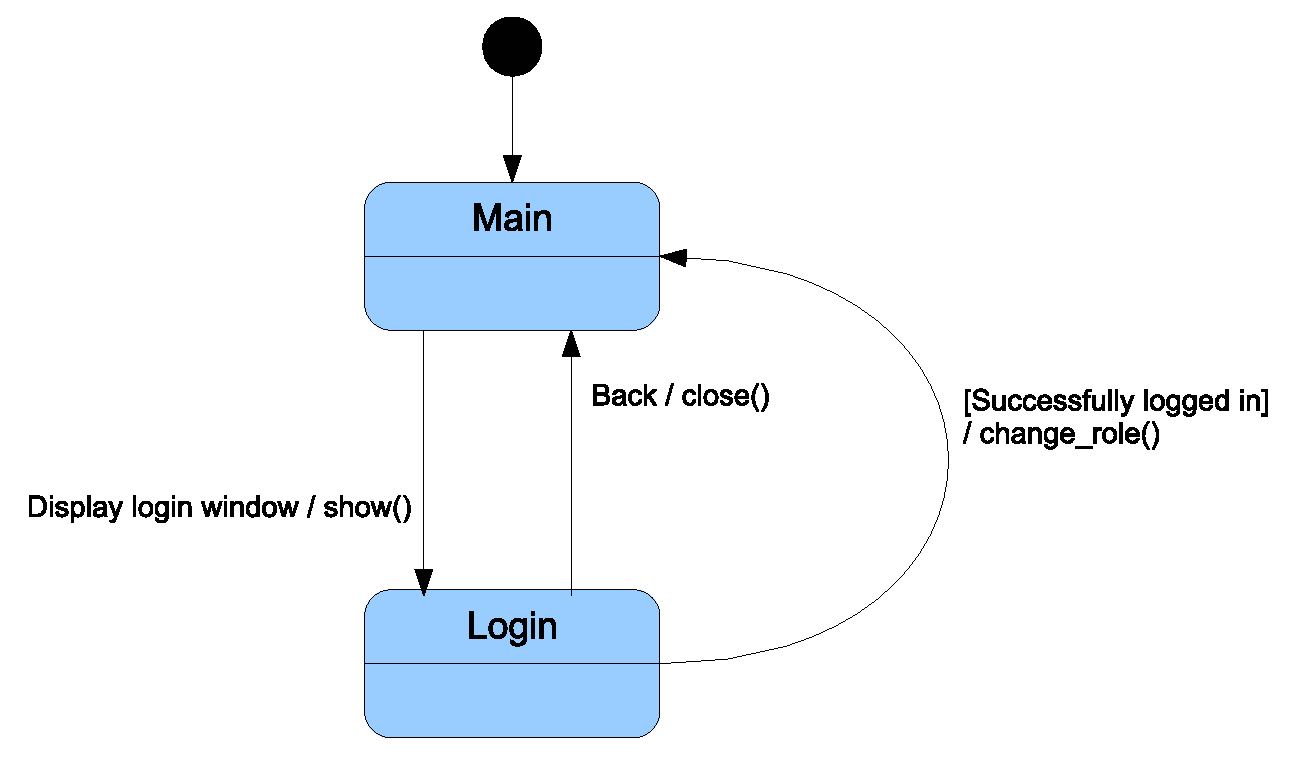
\includegraphics[width=9.5cm,keepaspectratio]{include/screens_role_visitor}
	\caption{Stavový diagram návaznosti obrazovek pro roli \uv{Návštěvník}}
	\label{fig:ScreensRoleVisitor}
\end{figure}

\begin{figure}[h]
	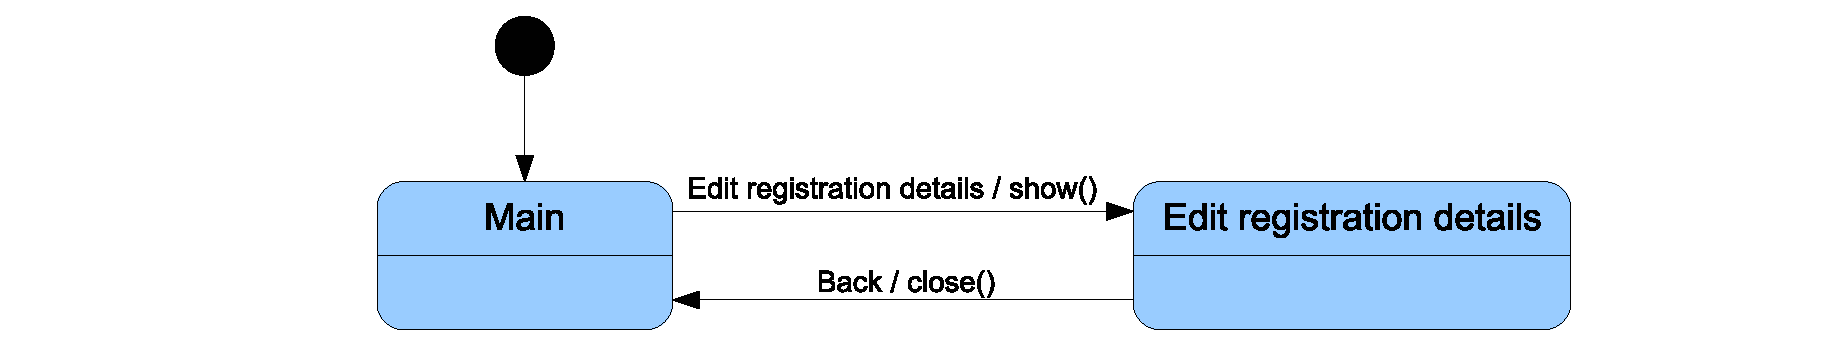
\includegraphics[width=12cm,keepaspectratio]{include/screens_role_registered}
	\caption{Stavový diagram návaznosti obrazovek pro roli \uv{Registrovaný}}
	\label{fig:ScreensRoleRegistered}
\end{figure}

\begin{figure}[h]
	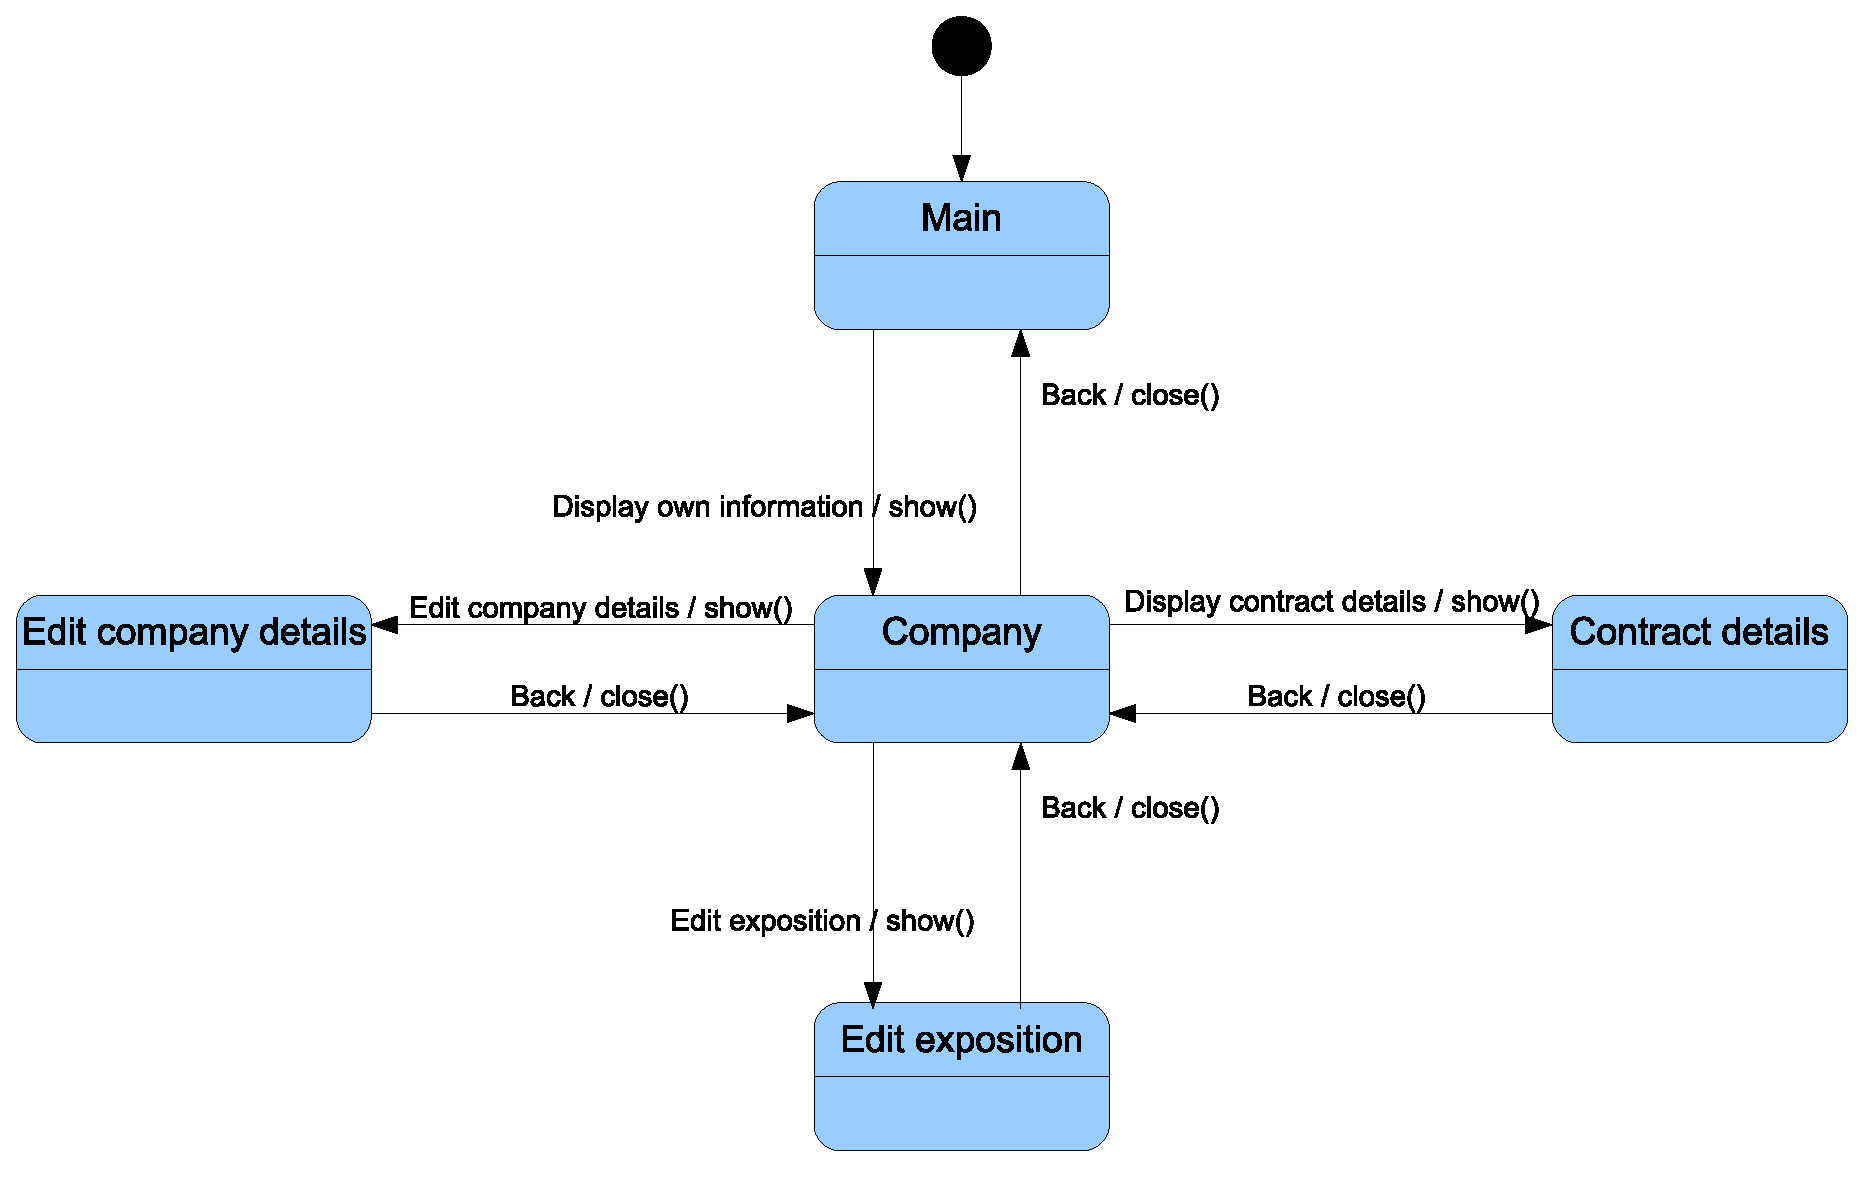
\includegraphics[width=11.8cm,keepaspectratio]{include/screens_role_firm}
	\caption{Stavový diagram návaznosti obrazovek pro roli \uv{Firma}}
	\label{fig:ScreensRoleFirm}
\end{figure}

\begin{figure}[h]
	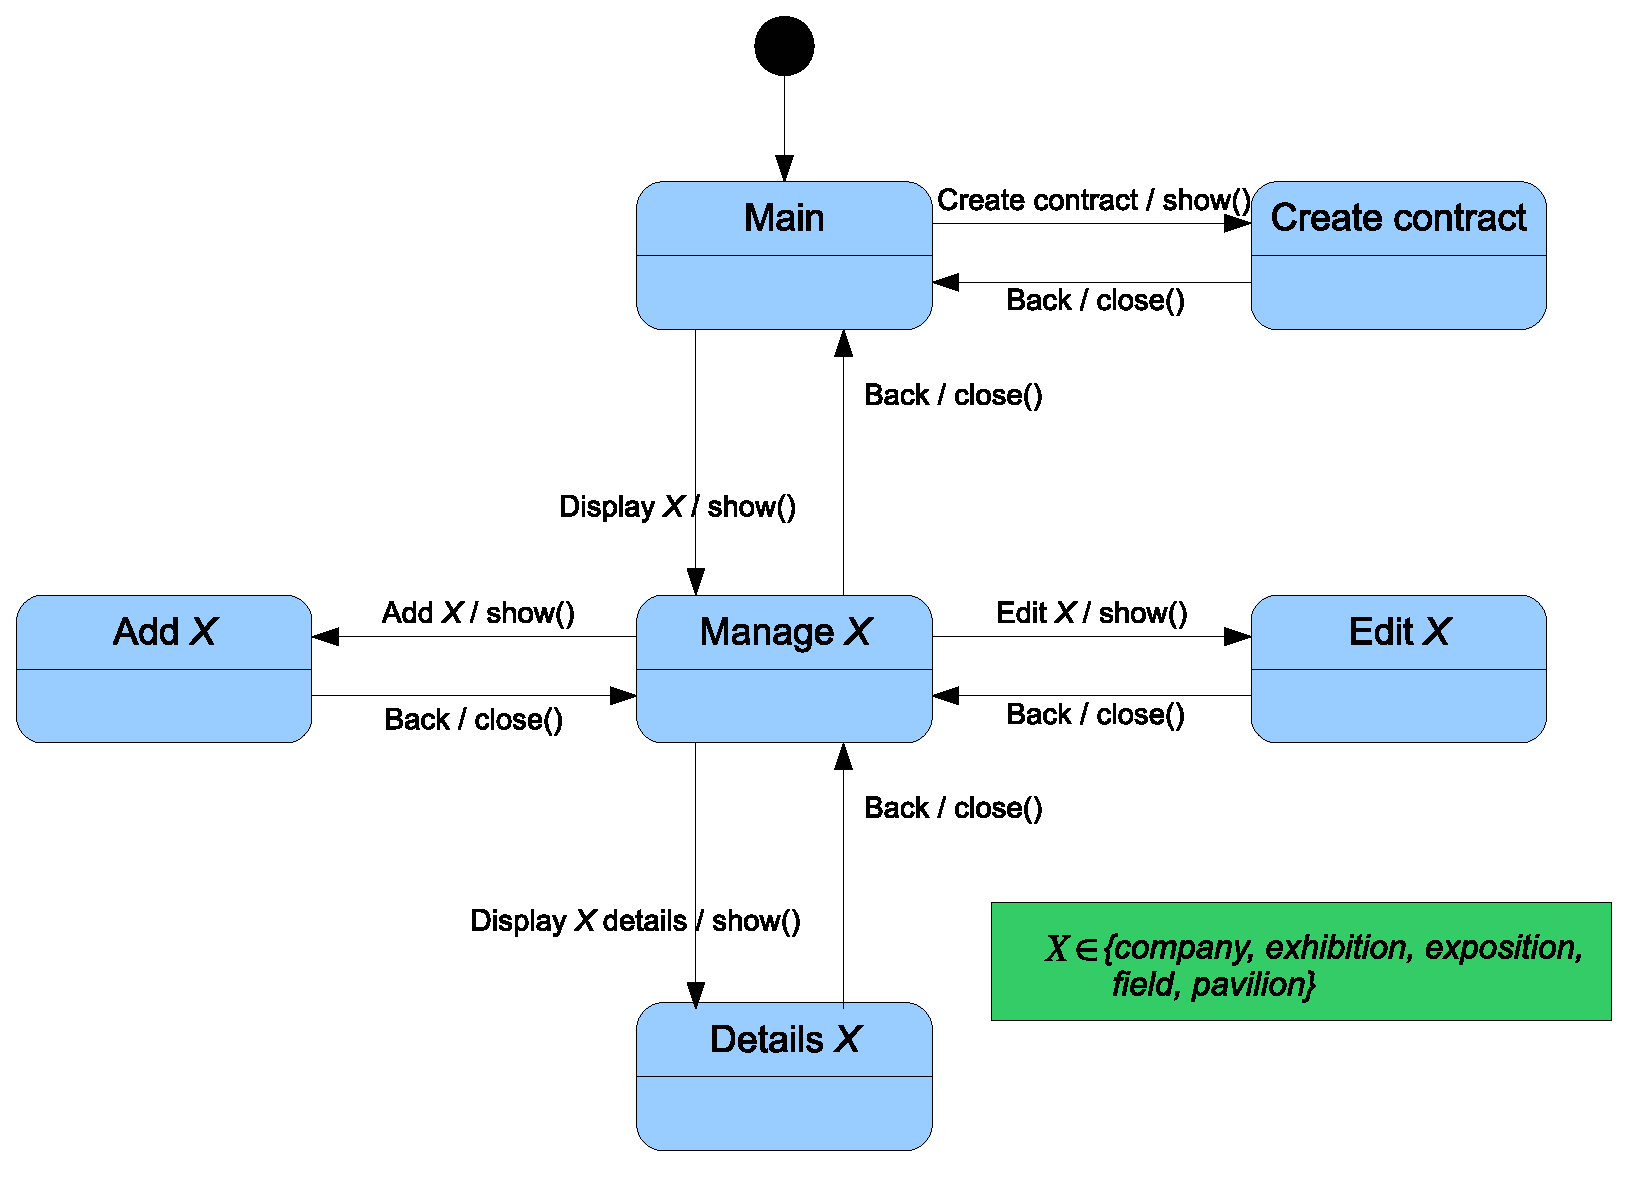
\includegraphics[width=11cm,keepaspectratio]{include/screens_role_employee}
	\caption{Stavový diagram návaznosti obrazovek pro roli \uv{Zaměstnanec}}
	\label{fig:ScreensRoleEmployee}
\end{figure}

\begin{landscape}
	\begin{figure}[h]
		\begin{center}
			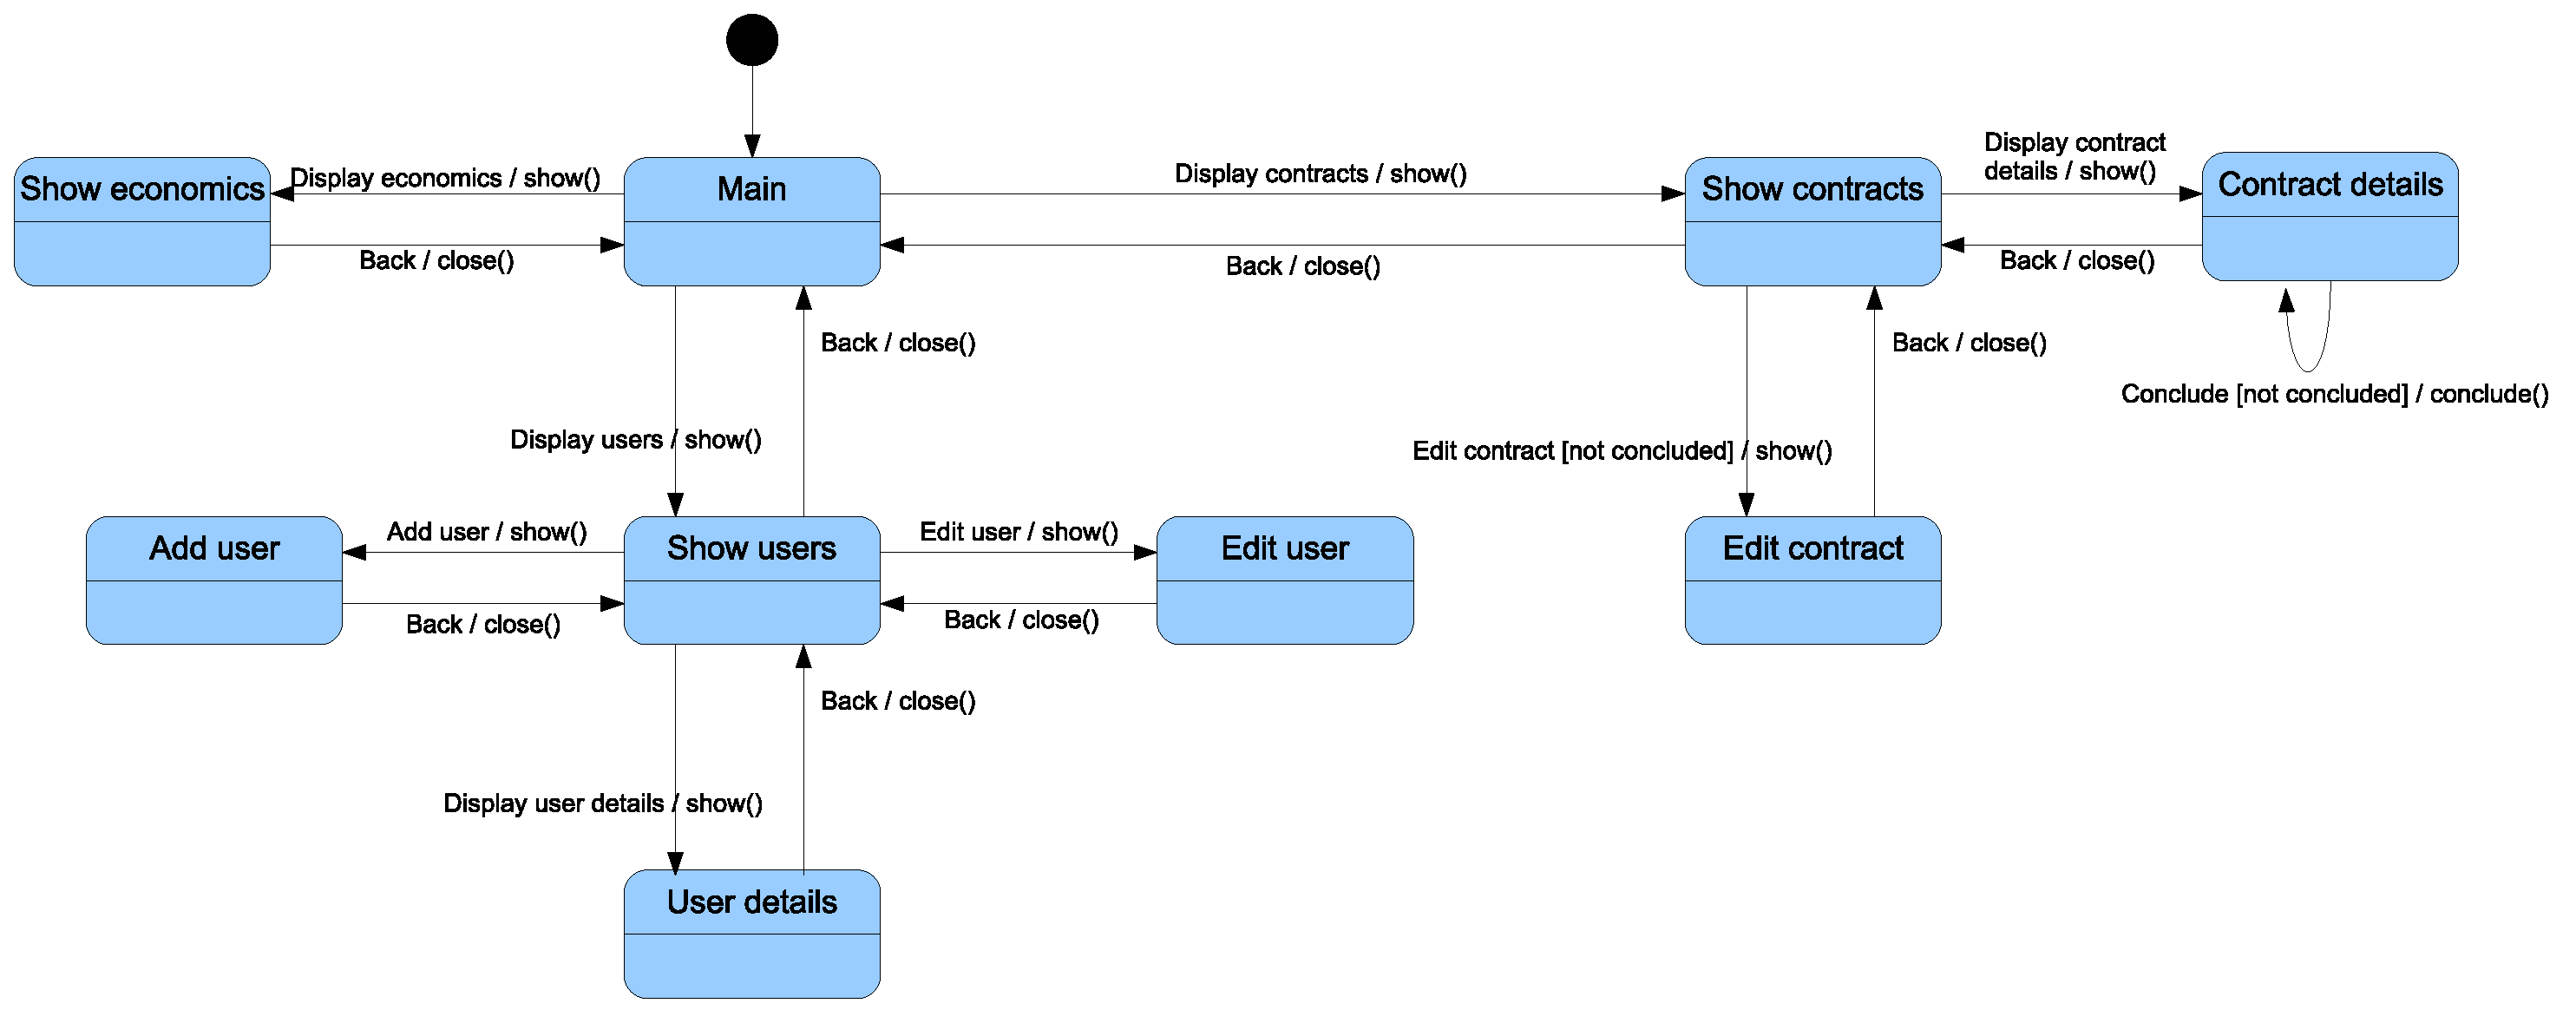
\includegraphics[width=26cm,keepaspectratio]{include/screens_role_chief}
		\end{center}
		\caption{Stavový diagram návaznosti obrazovek pro roli \uv{Vedoucí}}
		\label{fig:ScreensRoleChief}
	\end{figure}
\end{landscape}

\pagebreak

\section*{Grafické návrhy obrazovek}
\vspace{-2mm}
\begin{figure}[H]
	\begin{center}
		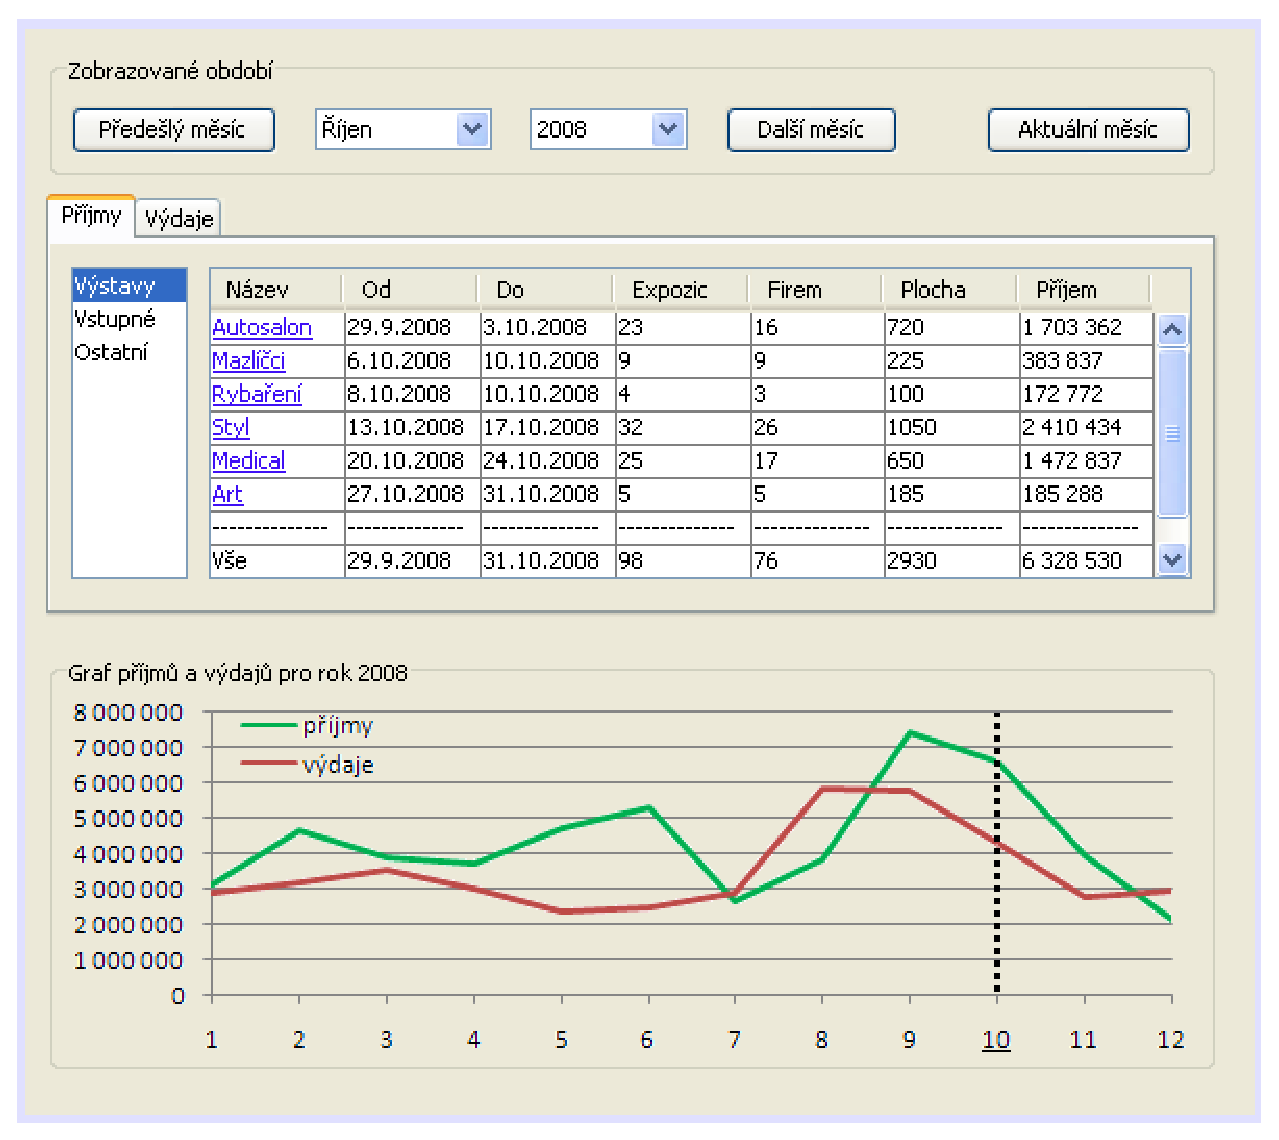
\includegraphics[width=11.85cm,keepaspectratio]{include/gui_econ_info}
	\end{center}
\vspace{-4mm}
	\caption{Grafický návrh obrazovky \uv{ekonomické informace}}
	\label{fig:GuiEconInfo}
\end{figure}
\vspace{-2mm}
\begin{figure}[H]
	\begin{center}
		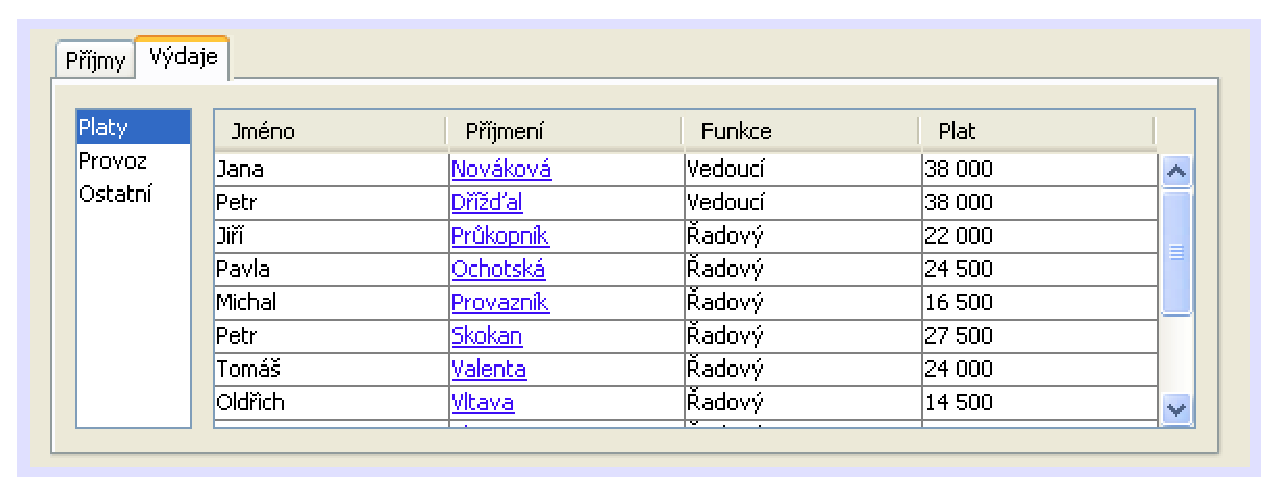
\includegraphics[width=11.85cm,keepaspectratio]{include/gui_econ_info2}
	\end{center}
\vspace{-4mm}
	\caption{Grafický návrh obrazovky \uv{ekonomické informace} - záložka výdaje}
	\label{fig:GuiEconInfo2}
\end{figure}

Poznámka: Pro možnost komplexní analýzy ekonomických informací by bylo vhodné systém propojit s~účetním programem.

\begin{figure}[H]
	\begin{center}
		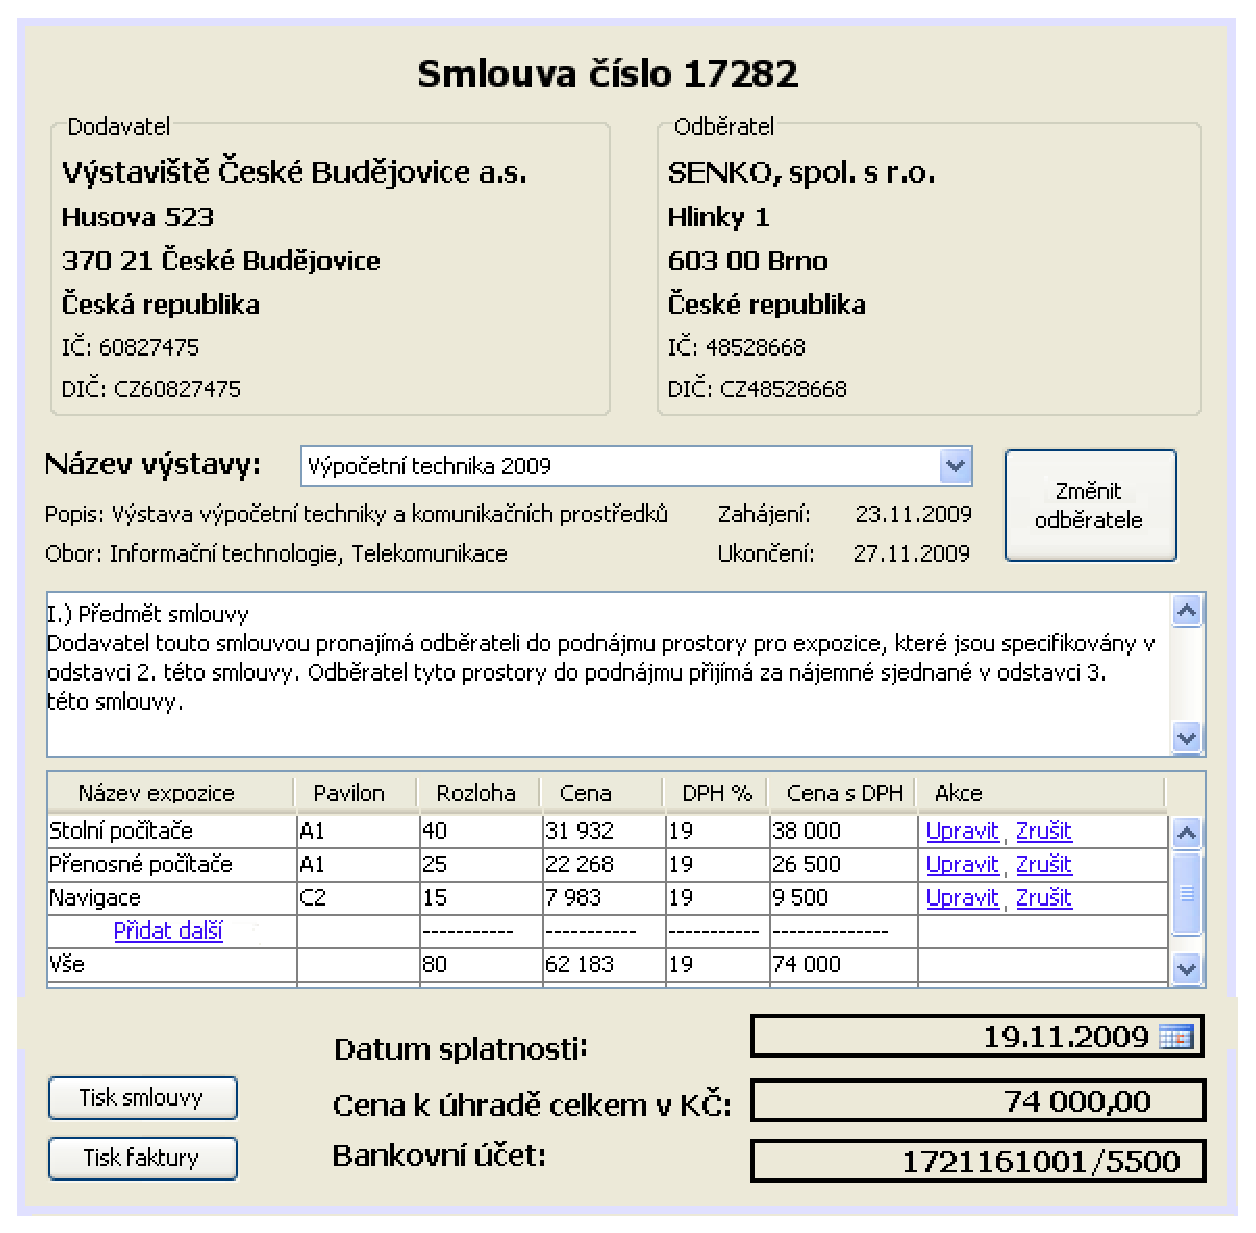
\includegraphics[width=11.6cm,keepaspectratio]{include/gui_contract}
	\end{center}
\vspace{-4mm}
	\caption{Grafický návrh obrazovky \uv{vytvoření smlouvy}}
	\label{fig:GuiContract}
\end{figure}

\begin{figure}[H]
	\begin{center}
		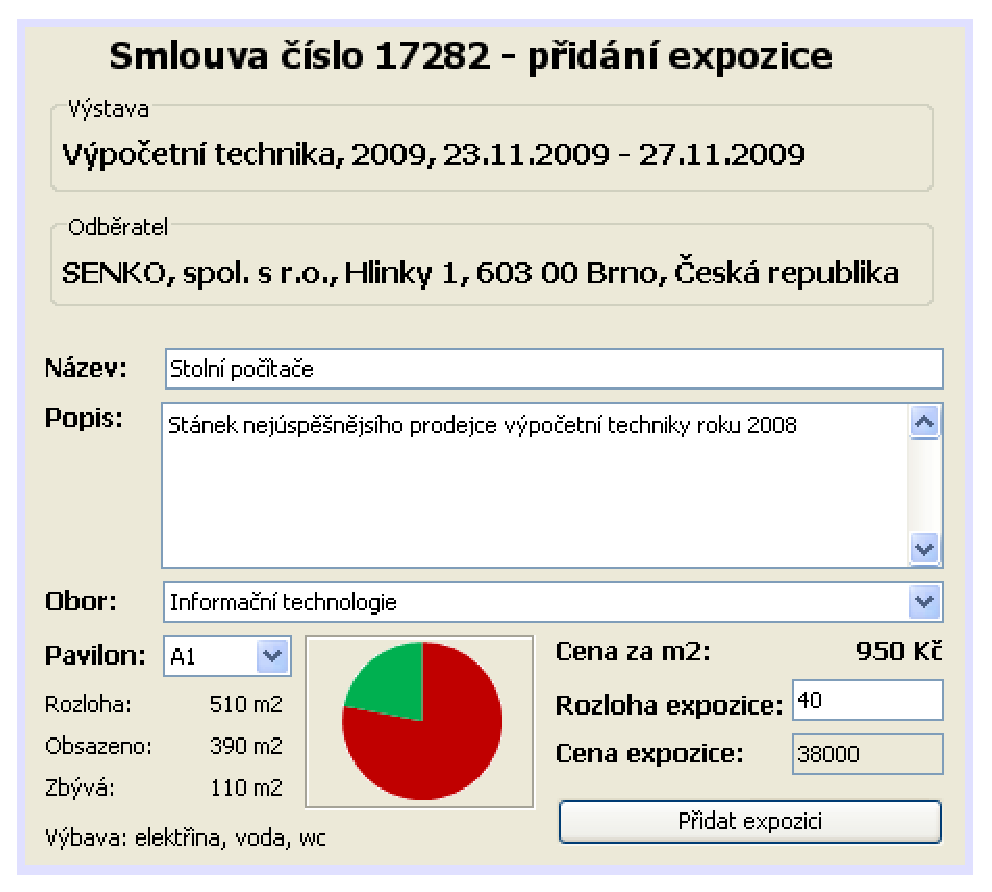
\includegraphics[width=9cm,keepaspectratio]{include/gui_contract2}
	\end{center}
\vspace{-4mm}
	\caption{Grafický návrh obrazovky \uv{vytvoření smlouvy} - přidání expozice}
	\label{fig:GuiContract2}
\end{figure}

\pagebreak

\section*{Přejímací testy}

\subsection*{Vyhledávání}

\begin{ais_table}
	\hline
	Popis: & Uživatel úspěšně vyhledává v~systému expozici podle části názvu a oboru \\

	\hline
	Předpoklady: &
		\begin{ais_table_first_enum}
			\item Uživatel se nachází v~hlavním okně programu

			\item V~systému se nachází expozice s~názvem \uv{Rybářské pruty LOTR 9000},
				která má přiřazen obor \uv{Rybolov}
		\end{ais_table_first_enum} \\

	\hline
	Postup: &
		\begin{ais_table_first_enum}
			\item Uživatel zvolí v~hlavním okně \uv{Hledat}

			\item Uživatel zadá slovo \uv{prut} do políčka \uv{Název expozice}

			\item Uživatel vybere ze seznamu oborů obor \uv{Rybolov}

			\item Uživatel potvrdí zadaná kritéria
		\end{ais_table_first_enum} \\

	\hline
	Úspěch: &
		\begin{ais_table_first_enum}
			\item Uživateli je vrácen seznam expozic, který obsahuje expozici
				s~názvem \uv{Rybářské pruty LOTR 9000} a přiřazeným oborem \uv{Rybolov}
		\end{ais_table_first_enum} \\

	\hline
\end{ais_table}

\subsection*{Vytvoření nové expozice}

\begin{ais_table}
	\hline
	Popis: & Zaměstnanec výstaviště úspěšně vytvoří novou expozici \\

	\hline
	Předpoklady: &
		\begin{ais_table_first_enum}
			\item Uživatel je přihlášen do systému jako zaměstnanec

			\item Uživatel má zobrazenou nepodepsanou smlouvu

			\item Uživatel má vybránu výstavu s~názvem \uv{EXPO 2014}, která trvá 9 dnů

			\item V~systému existuje obor s~názvem \uv{Rybolov}

			\item V~systému existuje pavilón \uv{E}, který má pro výstavu
				\uv{EXPO 2014} neobsazenou plochu nejméně $100\,m^{2}$ a cenu $299,-$\,Kč za $m^2$

			\item DPH pro pronájem expozice je nastaveno na 19\,\%
		\end{ais_table_first_enum} \\

	\hline
	Postup: &
		\begin{ais_table_first_enum}
			\item Uživatel v~seznamu expozic klikne na \uv{Přidat další}

			\item Zobrazí se okno \uv{Přidání nové expozice}

			\item Uživatel zadá název expozice \uv{Navijáky SW 4300} a popis expozice \uv{Ty nejpevnější navijáky na trhu}

			\item Uživatel vybere ze seznamu oborů \uv{Rybolov}

			\item Uživatel vybere ze seznamu pavilón \uv{E}

			\item Uživatel zadá rozlohu expozice $100\,m^{2}$
		\end{ais_table_first_enum} \\

	\hline
	Úspěch: &
		\begin{ais_table_first_enum}
			\item Uživateli se zobrazí smlouva, ke které přidával expozici

			\item V~seznamu expozic se nachází expozice s~názvem \uv{Navijáky SW 4300}, která je
				zamluvena pro výstavu \uv{EXPO 2014} a umístěna v~pavilónu \uv{E} s~rozlohou $100\,m^{2}$
				a celkovou cenou $269 100,-$\,Kč (bez DPH) a $320 229,-$\,Kč (s~DPH)

			\item Celková cena se zvedla o~$320 229,-$\,Kč (s~DPH)
		\end{ais_table_first_enum} \\

	\hline
\end{ais_table}

\subsection*{Přihlašování}

\begin{ais_table}
	\hline
	Popis: & Návštěvníkovi se nepodaří přihlásit do systému s~neplatným heslem \\

	\hline
	Předpoklady: &
		\begin{ais_table_first_enum}
			\item V~systému existuje uživatel s~přihlašovacím jménem \uv{Lucina},
				heslem \uv{Iiv3lohn} a jeho účet je nastaven jako aktivní
		\end{ais_table_first_enum} \\

	\hline
	Postup: &
		\begin{ais_table_first_enum}
			\item Návštěvník zvolí volbu \uv{Přihlásit}

			\item Návštěvník zadá přihlašovací jméno \uv{Lucina} a heslo \uv{pejsek}

			\item Návštěvník potvrdí zadané údaje kliknutím na tlačítko \uv{Přihlásit}
		\end{ais_table_first_enum} \\

	\hline
	Úspěch: &
		\begin{ais_table_first_enum}
			\item Návštěvníkovi je zobrazena chybová zpráva, která jej informuje o~tom,
				že zadané přihlašovací údaje jsou neplatné
		\end{ais_table_first_enum} \\

	\hline
\end{ais_table}

%%%%%%%%%%%%%%%%%%%%%%%%%%%%%%%%%%%%%%%%%%%%%%%%%%%%%%%%%%%%%%%%%%%%%%%%%%%%%%%
% vim: syntax=tex
%%%%%%%%%%%%%%%%%%%%%%%%%%%%%%%%%%%%%%%%%%%%%%%%%%%%%%%%%%%%%%%%%%%%%%%%%%%%%%%
